\documentclass[a4paper,10pt]{book}

\usepackage[usenames]{color}
\usepackage{bm}
\usepackage{amsmath}
\usepackage{xspace}
\usepackage{a4wide}
\usepackage{wrapfig}
\usepackage[numbers,comma,sort&compress]{natbib}
\usepackage{graphicx}
\usepackage{xstring}
\usepackage{listings,courier}
%\usepackage{draftcopy}
\usepackage{longtable}
\usepackage{paralist}
%\usepackage{fancyvrb}
\usepackage{listings}
\usepackage{array}
\usepackage[table]{xcolor}
\usepackage{units}
\usepackage[toc,page]{appendix}
\usepackage{lineno}
\usepackage{makeidx}

\definecolor{webgreen}{rgb}{0,.5,0}
\definecolor{webbrown}{rgb}{.6,0,0}
\definecolor{invisiblegray}{rgb}{.97,0.97,0.97}

\usepackage
[dvips, %dvipdf, %or dvips or pdftex 
pagebackref, %or backref
colorlinks=true,
linkcolor=webgreen, %defined below
filecolor=webbrown, %defined below
citecolor=webgreen, %defined below
pdftitle={VOTCA-CT manual},
pdfauthor={},
pdfsubject={VOTCA-CTP},
pdfkeywords={charge transport organic semiconductors},
bookmarksopen=false,
pdfpagemode=UseNone]{hyperref}

%\pdfcompresslevel=9

\usepackage[T1]{fontenc}
%\usepackage{times}
\usepackage{type1cm}
%\usepackage{showidx}

\def\bibsection{%
    \chapter*{Bibliography}%
    \addcontentsline{toc}{chapter}{Bibliography}
}

\makeindex

\begin{document}

\addtolength{\oddsidemargin}{-2cm}
\addtolength{\evensidemargin}{-2cm}
\addtolength{\textwidth}{0cm}
\addtolength{\topmargin}{0cm}
\addtolength{\textheight}{0cm}

\lstset{
  language=XML,
  frame=lines,
  backgroundcolor=\color{invisiblegray},
  basicstyle=\ttfamily\footnotesize,
  identifierstyle=\color{red},
  keywordstyle=\color{blue},
  commentstyle=\color{gray}\rmfamily\itshape,
  mathescape=true,
  morekeywords={estatic_params,estatic_method,epsilon_dielectric,s_eps}
}

\newcommand{\equ}[1]{eq.~\eqref{equ:#1}}
\newcommand{\Equ}[1]{Eq.~\eqref{equ:#1}}
\newcommand{\fig}[1]{figure~\ref{fig:#1}}
\newcommand{\Fig}[1]{Figure~\ref{fig:#1}}
\newcommand{\sect}[1]{section~\ref{sec:#1}}

\newcommand{\slink}[2]{\hyperref[sec:#1]{#2}}


\newcommand{\xml}{XML\xspace}
\newcommand{\gromacs}{GROMACS\xspace}
\newcommand{\gaussian}{GAUSSIAN\xspace}
\newcommand{\turbomole}{TURBOMOLE\xspace}
\newcommand{\tinker}{TINKER\xspace}

\newcommand{\Alq}{$\mathrm{Alq}_3$\xspace}
\newcommand{\dcvt}{DCV2T\xspace}

\newcommand{\xyz}{\texttt{geometry.xyz}\xspace}
\newcommand{\orb}{\texttt{zindo.orb}\xspace}
\newcommand{\votcactp}{{\MakeUppercase{votca-ctp}}\xspace}

\newcommand{\calculator}{\hyperref[sec:calculators]{calculator}\xspace}

\newcommand{\xmloptions}{\texttt{options.xml}\xspace}
\newcommand{\xmlcsg}{\texttt{map.xml}\xspace}
\newcommand{\xmlsegments}{\texttt{segments.xml}\xspace}
\newcommand{\sqlstate}{\texttt{state.db}\xspace}
\newcommand{\topology}{\texttt{topol.tpr}\xspace}
\newcommand{\trajectory}{\texttt{traj.xtc}\xspace}

\newcommand{\opt}{\texttt{{ -}-opt}\xspace}
\newcommand{\seg}{\texttt{{ -}-s}\xspace}
\newcommand{\sql}{\texttt{{ -}-db}\xspace}
\newcommand{\exe}{\texttt{{ -}-exec}\xspace}
\newcommand{\tpl}{\texttt{{ -}-top}\xspace}
\newcommand{\csg}{\texttt{{ -}-cg}\xspace}
\newcommand{\trj}{\texttt{{ -}-trj}\xspace}


\newcommand{\refcalc}{\hyperref[ref:calculators]{calculators}\xspace}

\newcommand{\overlap}{\hyperref[prog:moo_overlap]{\texttt{moo\_overlap}}\xspace}
\newcommand{\ctprun}{\hyperref[prog:ctp_run]{\texttt{ctp\_run}}\xspace}
\newcommand{\ctpmap}{\hyperref[prog:ctp_map]{\texttt{ctp\_map}}\xspace}

\newcommand{\ecoulomb}{\hyperref[calc:ecoulomb]{\texttt{ecoulomb}}\xspace}
\newcommand{\dumptraj}{\hyperref[calc:dumptraj]{\texttt{dumptraj}}\xspace}
\newcommand{\integrals}{\hyperref[calc:integrals]{\texttt{integrals}}\xspace}

\newcommand{\suggestion}[1]{{\color{red}SUGGESTION: #1}}

\newcommand{\segmentref}[1]{segments.#1}
\newcommand{\segmentopt}[1]{\hyperlink{\segmentref{#1}}{\StrSubstitute{#1}{_}{\_}}\xspace}
\newcommand{\calcref}[1]{#1}
\newcommand{\calcopt}[1]{\hyperlink{\calcref{#1}}{\StrSubstitute{#1}{_}{\_}}\xspace}

\newcommand{\calc}[1]{\hyperref[calc:#1]{\texttt{#1}}\xspace}



\frontmatter
\begin{titlepage}

%\center{\fontsize{4cm}{5cm}\selectfont VOTCA-CT}
%\center{\fontsize{1.5cm}{3cm}\selectfont USER MANUAL}

\center{\huge \sc VOTCA-CTP \\ \vspace*{1cm} Charge Transport Simulations}
\vspace*{1cm}
\center{\Large \sc User Manual}

\vspace*{3cm}
\center{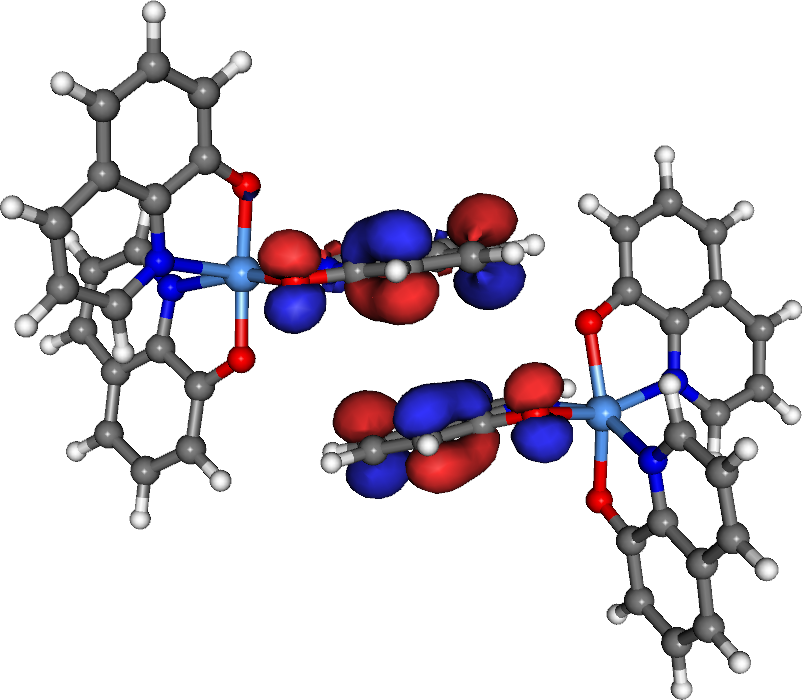
\includegraphics[width=0.6\columnwidth]{fig/logo}}
\vspace*{1cm}
\vfill

\center{\footnotesize{compiled from: \hgid}}
%\center{\footnotesize{Programs version: \refhgid}}
%\vspace*{1cm}
%\center{
%\large{\copyright \hspace*{0.1cm} VOTCA development team}
%}
\vspace*{0.5cm}
\center{\large{\today}} \\
\vspace*{0.3cm}
\htmladdnormallink{\color{black}\large{www.votca.org}}{http://www.votca.org}
\end{titlepage}

\section*{Disclamer}
The best way to start using the software is to look at provided tutorials. The reference section is generated automatically from the source code, so please make sure that your software and manual versions match.  

\section*{Citations}
Development of this software depends on academic research grants. If you are using the package, please cite the  following papers \\

\vspace{0.1cm}
\noindent
\cite{poelking_long-range_2016} Long-range embedding of molecular ions and excitations in a polarizable molecular environment, \\
Carl Poelking and Denis Andrienko \\
\htmladdnormallink{  {\itshape J. Chem. Theory Comp.} 12, 4516-4523, 2016}
{http://dx.doi.org/10.1021/acs.jctc.6b00599} \\

\vspace{0.1cm}
\noindent
\cite{ruhle_microscopic_2011} Microscopic simulations of charge transport in disordered organic semiconductors, \\
Victor R\"uhle, Alexander Lukyanov, Falk May, Manuel Schrader, Thorsten Vehoff, James Kirkpatrick, Bj\"orn Baumeier and Denis Andrienko \\
\htmladdnormallink{  {\itshape J. Chem. Theor. Comp.} 7, 3335, 2011}
{http://dx.doi.org/10.1021/ct200388s} \\

\vspace{0.1cm}
\noindent
\cite{ruhle_versatile_2009} Versatile Object-oriented Toolkit for Coarse-graining Applications \\
Victor R\"uhle, Christoph Junghans, Alexander Lukyanov, Kurt Kremer and Denis Andrienko \\
\htmladdnormallink{  {\itshape J. Chem. Theor. Comp.} 5, 3211, 2009}
{http://dx.doi.org/10.1021/ct900369w}

\section*{Development}
The core development is currently taking place at the Max Planck Institute for Polymer Research, Mainz, Germany.

\section*{Copyright}
\votcactp is free software. The entire package is available under the Apache License. For details, check
the LICENSE file in the source code. The \votcactp source code is available on our homepage, \htmladdnormallink{\color{black}www.votca.org}{http://www.votca.org}.

\vfill

\thispagestyle{empty}
\cleardoublepage

\tableofcontents
%\cleardoublepage
\mainmatter

\printindex
\linenumbers

\chapter{Introduction}
\label{sec:introduction}

Charge carrier dynamics in an organic semiconductor can often be described in terms of charge hopping between localized states. The hopping rates depend on \slink{sec:transfer_integrals}{electronic coupling elements}, \slink{sec:reorganization}{reorganization energies}, and \slink{sec:site_energies}{site energies}, which vary as a function of position and orientation of the molecules. 
%The exact evaluation of these contributions in a molecular assembly is computationally prohibitive. Various, often semi-empirical, approximations are employed instead. 
The purpose of the \votcactp package~\cite{ruhle_microscopic_2011} is to simplify the workflow for charge transport simulations, provide a uniform error-control for the methods, flexible platform for their development, and eventually allow {\em in silico} prescreening of organic semiconductors for specific applications. 

The toolkit is implemented using modular concepts introduced earlier in the Versatile Object-oriented Toolkit for Coarse-graining Applications (VOTCA)~\cite{ruhle_versatile_2009}. It contains different \slink{sec:programs}{programs}, which execute specific tasks implemented in \slink{sec:calculators}{calculators} representing an individual step in the workflow. \Fig{summary} summarizes a typical chain of commands to perform a charge transport simulation:   
%
First, the VOTCA code structures are adap\-ted to reading atomistic trajectories, mapping them onto \slink{segments}{conjugated segments and rigid fragments}, and substituting (if needed) rigid fragments with the optimized copies (\ctpmap). The programs \ctprun and \ctpparallel (for heavy-duty tasks) are then used to calculate all bimolecular charge hopping rates (via precalculation of all required ingredients). \slink{sec:site_energies}{Site energies (or energetic disorder)} can be determined as a combination of internal (ionization potentials/electron affinities of single molecules) as well as electrostatic and polarization contributions with in the molecular environment. The calculation of \slink{sec:transfer_integrals}{electronic coupling elements} between conjugated segments from the corresponding molecular orbitals can be performed using a \slink{sec:dipro}{dimer-projection} technique based on \slink{sec:dft}{density-functional} theory (DFT). This requires explicit calculations using quantum-chemistry software for which we provide interfaces to \gaussian, \turbomole, and \nwchem. Alternatively, the \slink{sec:izindo}{molecular orbital overlap} module calculates electronic coupling elements relying on the semi-empirical INDO Hamiltonian and molecular orbitals in the format provided by the \gaussian package. 

The  \slink{sec:kmc}{kinetic Monte Carlo} module reads in the \slink{neighborlist}{neighbor list}, \slink{morphology}{site coordinates}, and \slink{rates}{hopping rates} and performs charge dynamics simulations using either periodic boundary conditions or charge sources and sinks. 

The toolkit is written as a combination of modular C++ code and scripts. The data transfer between programs is implemented via a \slink{statefile}{state file} (sql database), which is also used to restart simulations. Analysis functions and most of the calculation routines are encapsulated by using the observer pattern~\cite{gamma_design_1995} which allows the implementation of new functions as individual modules.

In the following \sect{theory}, we summarize the \slink{sec:theory}{theoretical background} of the workflow of charge transport simulations and i partciular its individual steps. \Sect{io} describes the structure and content of input and output files, while a full reference of \slink{sec:programs}{programs} and \slink{sec:calculators}{calculators} is available in \sect{reference}. For a hands-on tutorial, the reader is referred to the \hyperref[http://code.google.com/p/votca-ctp/]{\votcactp} project page at http://code.google.com/p/votca-ctp/.



\tikzstyle{decision} = [diamond, draw, fill=mygray]
\tikzstyle{line} = [draw, -stealth, thick]
\tikzstyle{block} = [draw, rectangle, fill=mygray, text width=0.5\linewidth]
\tikzstyle{smallblock} = [draw, rectangle, fill=mygray, text width=0.4\linewidth]
\tikzstyle{info} = [text width=0.35\linewidth]
\tikzstyle{smallinfo} = [text width=0.25\linewidth]
\tikzstyle{biginfo} = [text width=0.9\linewidth]
\begin{figure}
\centering
\newcommand{\vgap}{0.5cm}
\begin{scriptsize}
\noindent\begin{tikzpicture}
\node [block] (mapping) {{\bf Mapping}\\Converts and partitions atomistic \gromacs trajectory \vskip 0.1cm
{\noindent  \cmdmap}
\vskip 0.1cm};

\node[smallinfo, left=0.0 of mapping] (input) {{\bf Input files:}\\\texttt{conf.gro}\\\,\hskip 0.1cm\gromacs trajectory\\\texttt{topol.tpr}\\\hskip0.1cm\gromacs topology\\\texttt{\xmlcsg}\\\hskip0.1cm mapping and energies\\\texttt{options.xml}\\\hskip0.1cm options for \slink{sec:calculators}{calculators}\vskip 0.2cm {\bf Output files:}\\\texttt{\sqlstate}\\\hskip0.1cm \sqlite database file for\\\hskip0.1cm data transfer between\\\hskip0.1cm modules};

\node [block, below=\vgap of mapping] (nbl) {{\bf Neighbor list}\\Indentifies close molecular pairs between which charge transfer rates will be calculated \vskip 0.1cm
{\noindent \cmdnbl}
\vskip 0.1cm};


\node [block, below=\vgap of nbl] (site_energies) {{\bf Site energies}\\Calculates electrostatic and polarization contribution to site energies \vskip 0.1cm
{\noindent  \cmdemlt} };

\node [block, below=\vgap of site_energies] (int_energies) {{\bf Internal site and reorganization energies}\\Imports internal site energy (IP, EA) and reorganization energies for charging and discharging to \sqlstate \vskip 0.1cm
{\noindent  \cmdeint}
\vskip 0.1cm};


% above right=0.7cm and 4cm of A
\node[decision, below=\vgap of int_energies](decision1){Transfer integrals};

%\node (AuxNode01) [text width=6em, below of = decision1, node distance=7em ] {};

\node [smallblock, below left=\vgap of decision1] (DFT_TI) {{\bf Monomers with DFT}\\Calculate the relevant transport orbitals of monomers \vskip 0.1cm
{ \cmdedft \job\, ''\wrt \run'' }};

\node [smallblock, below=\vgap of DFT_TI] (DFT_TI2) {{\bf Transfer integrals with DFT}\\Calculate electronic coupling elements for all pairs in the neighbor list \vskip 0.1cm
{ \cmdidft \job\, ''\wrt \run \rd'' }
\vskip 0.1cm};

\node [smallblock, below right=\vgap of decision1] (DFT_ZINDO) {{\bf Transfer integrals with ZINDO}\\Calculate electronic coupling elements for all pairs in the neighbor list  \vskip 0.1cm
{\noindent  \cmdizindo }
\vskip 0.1cm};


\node[info, below=0.2cm of DFT_ZINDO] (ti_info) {{One can choose between quantum-chemical (computationally expensive) or semi-empirical (fast, but not always sufficiently accurate) evaluation of transfer integrals.}};

\node (AuxNode01) [below=\vgap of DFT_TI2, xshift=0.25\linewidth] {};


\node [block, below=\vgap of DFT_TI2, xshift=0.275\linewidth] (outer_reorg) {{\bf Outersphere reorganization energies}\\Contribution to reorganization of surrounding molecules due to polarization. (optional for Marcus rates)  \vskip 0.1cm
{\noindent  \cmdouter}
\vskip 0.1cm};

\node [block, below=\vgap of outer_reorg] (rates) {{\bf Charge transfer rates}\\Calculates rates for charge transfer among all pairs in the neighborlist \vskip 0.1cm
{\noindent \cmdrates}
};

\node [block, below=\vgap of rates] (kmc) {{\bf Charge dynamics via kMC}\\Hopping of charge carriers simulated via kinetic Monte Carlo \vskip 0.1cm
{\noindent \cmdkmc }
};

\node [biginfo, below=\vgap of kmc] (calc) {{\noindent Get list of available calculators: \ctprun/\ctpparallel/\kmcrun  \texttt{ -l}}\\ Get help and list of options for a calculator: \ctprun/\ctpparallel/\kmcrun  \texttt{ -d }\calc{neighborlist}};

\path [line] (mapping) -- (nbl);
\path [line] (nbl) -- (site_energies);
\path [line] (site_energies) -- (int_energies);
\path [line] (int_energies) -- (decision1);
\path [line] (DFT_TI) -- (DFT_TI2);
\path [line] (decision1) -| node[yshift=0.5em, xshift=1em] {DFT} (DFT_TI);
\path [line] (decision1) -| node[yshift=0.5em, xshift=-1em] {ZINDO} (DFT_ZINDO);
\path [line] (DFT_TI2.east) -| (outer_reorg.north);
\path [line] (DFT_ZINDO.west) -| (outer_reorg);
\path [line] (outer_reorg) -- (rates);
\path [line] (rates) -- (kmc);
\end{tikzpicture}


\end{scriptsize}
\caption{A practical workflow of charge transport simulations using \votcactp. The \slink{sec:theory}{theoretical background} of the individual steps is given in \sect{theory}. \Sect{io} describes the content of input and output files, while a full reference of \slink{sec:programs}{programs} and \slink{sec:calculators}{calculators} is available in \sect{reference}.  }
\label{fig:summary}
\end{figure}

\chapter{Theoretical background}
\label{sec:theory}
\section{Workflow}
\label{sec:wokflow}

A typical workflow of charge transport simulations is depicted in \fig{workflow}. The first step is the simulation of an \slink{morphology}{atomistic morphology}, which is then partitioned on \slink{segments}{hopping sites}. The coordinates of the hopping sites are used to construct a list of pairs of molecules, or \slink{neighborlist}{neighbor list}. 

\begin{figure}[h]
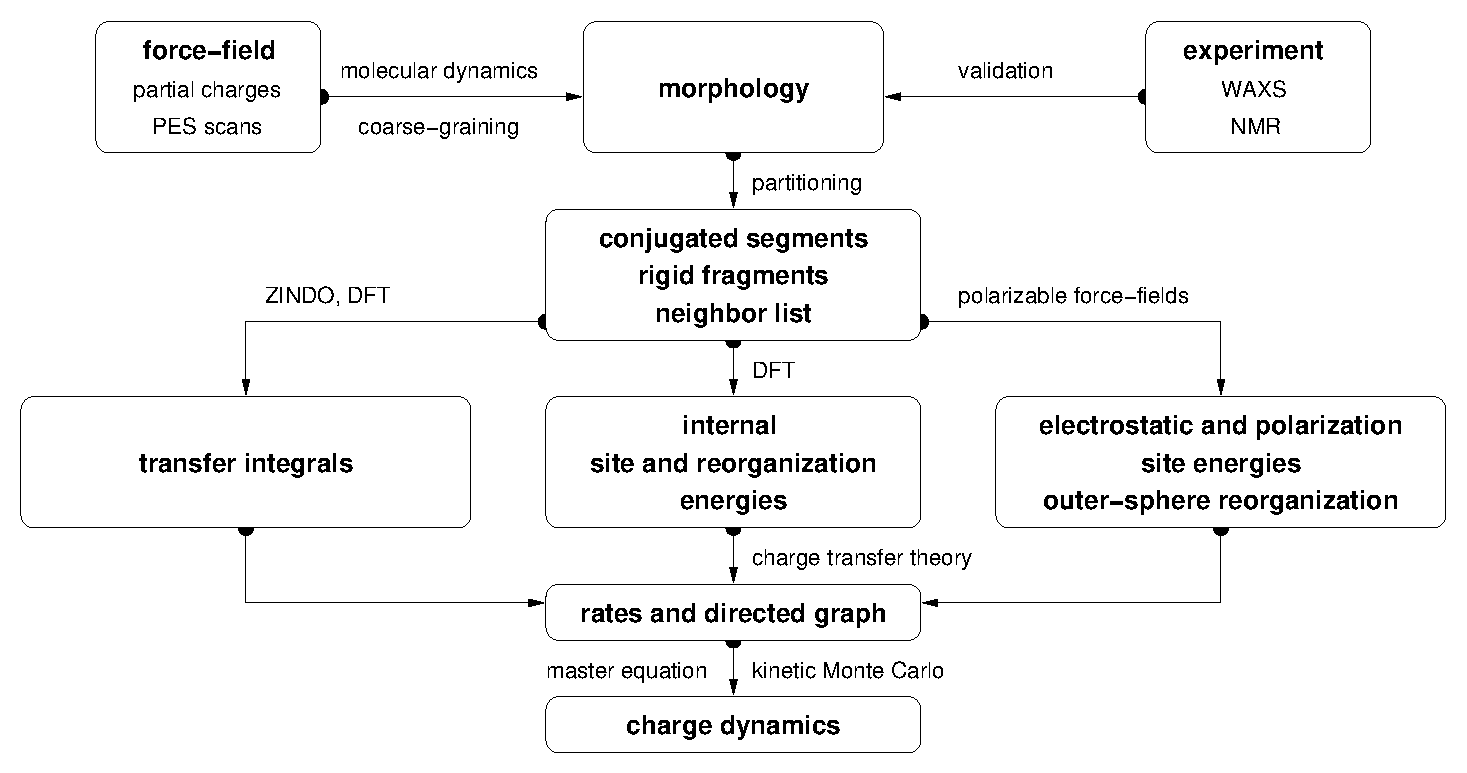
\includegraphics[width=\textwidth]{fig/workflow/workflow}
 \caption{%
   Workflow for microscopic simulations of charge transport.  %
   \label{fig:workflow}}
\end{figure}

For each pair an \slink{transfer_integrals}{electronic coupling element}, a \slink{reorganization}{reorganization energy}, a \slink{site_energies}{driving force}, and eventually the \slink{rates}{hopping rate} are evaluated. The neighbor list and hopping rates define a directed graph. The corresponding master equation is solved using the \slink{kmc}{kinetic Monte Carlo} method, which allows to explicitly monitor the charge dynamics in the system as well as to calculate time or ensemble averages of occupation probabilities, charge fluxes, correlation functions, and field-dependent mobilities.


\begin{figure}[p]
\includegraphics[width=\textwidth]{fig/workflow_practical/workflow_practical}
 \caption{%
   Workflow for microscopic simulations of charge transport including calls.  %
   \label{fig:workflow}}
\end{figure}


\tikzstyle{decision} = [diamond, draw, fill=blue!50]
\tikzstyle{line} = [draw, -stealth, thick]
\tikzstyle{elli}=[draw, ellipse, fill=red!50,minimum height=8mm, text width=5em ]
\tikzstyle{block} = [draw, rectangle, fill=blue!50, text width=\linewidth]
\tikzstyle{smallblock} = [draw, rectangle, fill=blue!50, text width=0.4\linewidth]
\begin{figure}
\centering
\newcommand{\vgap}{0.5cm}
\begin{footnotesize}
\noindent\begin{tikzpicture}
\node [block] (mapping) {{\bf Mapping}\\Converts and partitions atomistic \gromacs trajectory \vskip 0.1cm
{\noindent  \ctpmap \tpl \topology \trj \trajectory \seg \xmlcsg  \sql \sqlstate}
\vskip 0.1cm};

\node [block, below=\vgap of mapping] (nbl) {{\bf Neighbor list}\\Indentifies close molecular pairs between which charge transfer rates will be calculated \vskip 0.1cm
{\noindent  \ctprun \opt \xmloptions  \seg  \xmlsegments \sql  \sqlstate \exe  \calc{neighborlist}}
\vskip 0.1cm};


\node [block, below=\vgap of nbl] (site_energies) {{\bf Site energies}\\Calculates electrostatic and polarization contribution to site energies \vskip 0.1cm
{\noindent  \ctprun \opt \xmloptions  \sql  \sqlstate \exe  \calc{emultipole} } };

\node [block, below=\vgap of site_energies] (int_energies) {{\bf Internal site and reorganization energies}\\Imports internal site energy (IP, EA) and reorganization energies for charging and discharging to \sqlstate \vskip 0.1cm
{\noindent  \ctprun \opt \xmloptions  \sql  \sqlstate \exe  \calc{einternal} }
\vskip 0.1cm};


% above right=0.7cm and 4cm of A
\node[decision, below=\vgap of int_energies](decision1){Transfer integrals};

%\node (AuxNode01) [text width=6em, below of = decision1, node distance=7em ] {};

\node [smallblock, below left=\vgap of decision1] (DFT_TI) {{\bf Monomers with DFT}\\Calculate the relevant transport orbitals of monomers\\ prepare job file \vskip 0.1cm
{ \ctpparallel \opt \xmloptions \sql \sqlstate \exe \calc{edft} \job \wrt }
\vskip 0.1cm execute jobs \vskip 0.1cm
{ \ctpparallel \opt \xmloptions \sql \sqlstate \exe \calc{edft} \job \run }
};

\node [smallblock, below=\vgap of DFT_TI] (DFT_TI2) {{\bf Electronic coupling with DFT}\\Calculate electronic coupling elements for all pairs in the neighbor list \vskip 0.1cm
{ \ctpparallel \opt \xmloptions \sql \sqlstate \exe \calc{idft} \job `` \wrt \run \rd\'' }
\vskip 0.1cm};

\node [smallblock, below right=\vgap of decision1] (DFT_ZINDO) {{\bf Electronic coupling with ZINDO}\\Imports internal site energy (IP, EA) and reorganization energies for charging and discharging to \sqlstate \vskip 0.1cm
{\noindent  \ctprun \opt \xmloptions  \sql  \sqlstate \exe  \calc{einternal} }
\vskip 0.1cm};

\node (AuxNode01) [below=\vgap of DFT_TI2, xshift=0.25\linewidth] {};


\node [block, below=\vgap of DFT_TI2, xshift=0.275\linewidth] (outer_reorg) {{\bf Outersphere reorganization energies}\\Imports internal site energy (IP, EA) and reorganization energies for charging and discharging to \sqlstate \vskip 0.1cm
{\noindent  \ctprun \opt \xmloptions  \sql  \sqlstate \exe  \calc{outersphere} }
\vskip 0.1cm};

\node [block, below=\vgap of outer_reorg] (rates) {{\bf Charge transfer rates}\\Calculates rates for charge transfer among all pairs in the neighborlist \vskip 0.1cm
{\noindent \small \ctprun \opt \xmloptions \sql  \sqlstate \exe  \calc{rates} }
};

\node [block, below=\vgap of rates] (kmc) {{\bf Charge dynamics via kMC}\\Hopping of charge carriers simulated via kinetic Monte Carlo \vskip 0.1cm
{\noindent  \kmcrun \opt \xmloptions  \sql  \sqlstate \exe  \calc{kmcmultiple} }
};
%%
%(ClOp.west) -- ++(-0.2,0) -- ([yshift=0.5cm, xshift=-0.2cm] Pressure.north west) -|
%     ([xshift=-1cm]Sensor.south);
%    \draw[myarrow] (Ammeter.east) -- ++(0.2,0) -- ([yshift=0.5cm, xshift=0.2cm] Temperature.north east) -|
%     ([xshift=1cm]Sensor.south);

%\node [block, left of=mapping, xshift=-5em] (nbl) {Process 1};
%\node [elli, above of=mapping, yshift=5em] (user) {user};
%\node [block, right of=mapping, xshift=5em] (process2) {Process 2};
%\node[decision, below of=mapping, yshift=-5em](decision1){Process 1?};
%arrows
%\path [line] (user) -- (mapping);
\path [line] (mapping) -- (nbl);
\path [line] (nbl) -- (site_energies);
\path [line] (site_energies) -- (int_energies);
\path [line] (int_energies) -- (decision1);
\path [line] (DFT_TI) -- (DFT_TI2);
\path [line] (decision1) -| node[yshift=0.5em, xshift=1em] {DFT} (DFT_TI);
\path [line] (decision1) -| node[yshift=0.5em, xshift=-1em] {ZINDO} (DFT_ZINDO);
\path [line] (DFT_TI2) -- (outer_reorg);
\path [line] (DFT_ZINDO) -- (outer_reorg);
\path [line] (outer_reorg) -- (rates);
\path [line] (rates) -- (kmc);
\end{tikzpicture}


\end{footnotesize}
\caption{LALA}
\end{figure}


\section{Material morphology}
\label{sec:morphology}

There is no generic recipe on how to predict a large-scale atomistically-resolved morphology of an organic semiconductor. The required methods are system-specific: for ultra-pure crystals, for example, density-functional methods can be used provided the crystal structure is known from experiment. For partially disordered organic semiconductors, however, system sizes much larger than a unit cell  are required. Classical molecular dynamics or Monte Carlo techniques are then the methods of choice. 

In molecular dynamics, atoms are represented by point masses which interact via empirical potentials prescribed by a force-field. Force-fields are parametrized for a limited set of compounds and their refinement is often required for new molecules. In particular, special attention shall be paid to torsion potentials between successive repeat units of conjugated polymers or between functional groups and the $\pi$-conjugated system. First-principles methods can be used to characterize the missing terms of the potential energy function. 

Self-assembling materials, such as soluble oligomers, discotic liquid crystals, block copolymers, partially crystalline polymers, etc., are the most complicated to study. The morphology of such systems often has several characteristic length scales and can be kinetically arrested in a thermodynamically non-equilibrium state. For such systems, the time- and length-scales of atomistic simulations might be insufficient to equilibrate or sample desired morphologies. In this case, systematic coarse-graining can be used to enhance sampling~\cite{ruehle_versatile_2009}. Note that the coarse-grained representation must reflect the structure of the atomistic system and allow for back-mapping to the atomistic resolution.

Here we assume that the morphology is already known, that is we know how the topology and the coordinates of all atoms in the systems at a given time. \votcact can read standard \gromacs topology files. Custom definitions of \hyperref[sec:atomistic]{atomistic topology} via \xml files are also possible. Since the description of the atomistic topology is the first step in the charge transport simulations, it is important to follow simple conventions on how the system is partitioned on molecules, residues, and how atoms are named in the topology. Required input files are described in section \hyperref[sec:atomistic]{Atomistic topology}. 


\section{Conjugated segments and rigid fragments}
\label{sec:conjugated_segments}

\begin{wrapfigure}{ht}{0.5\linewidth}
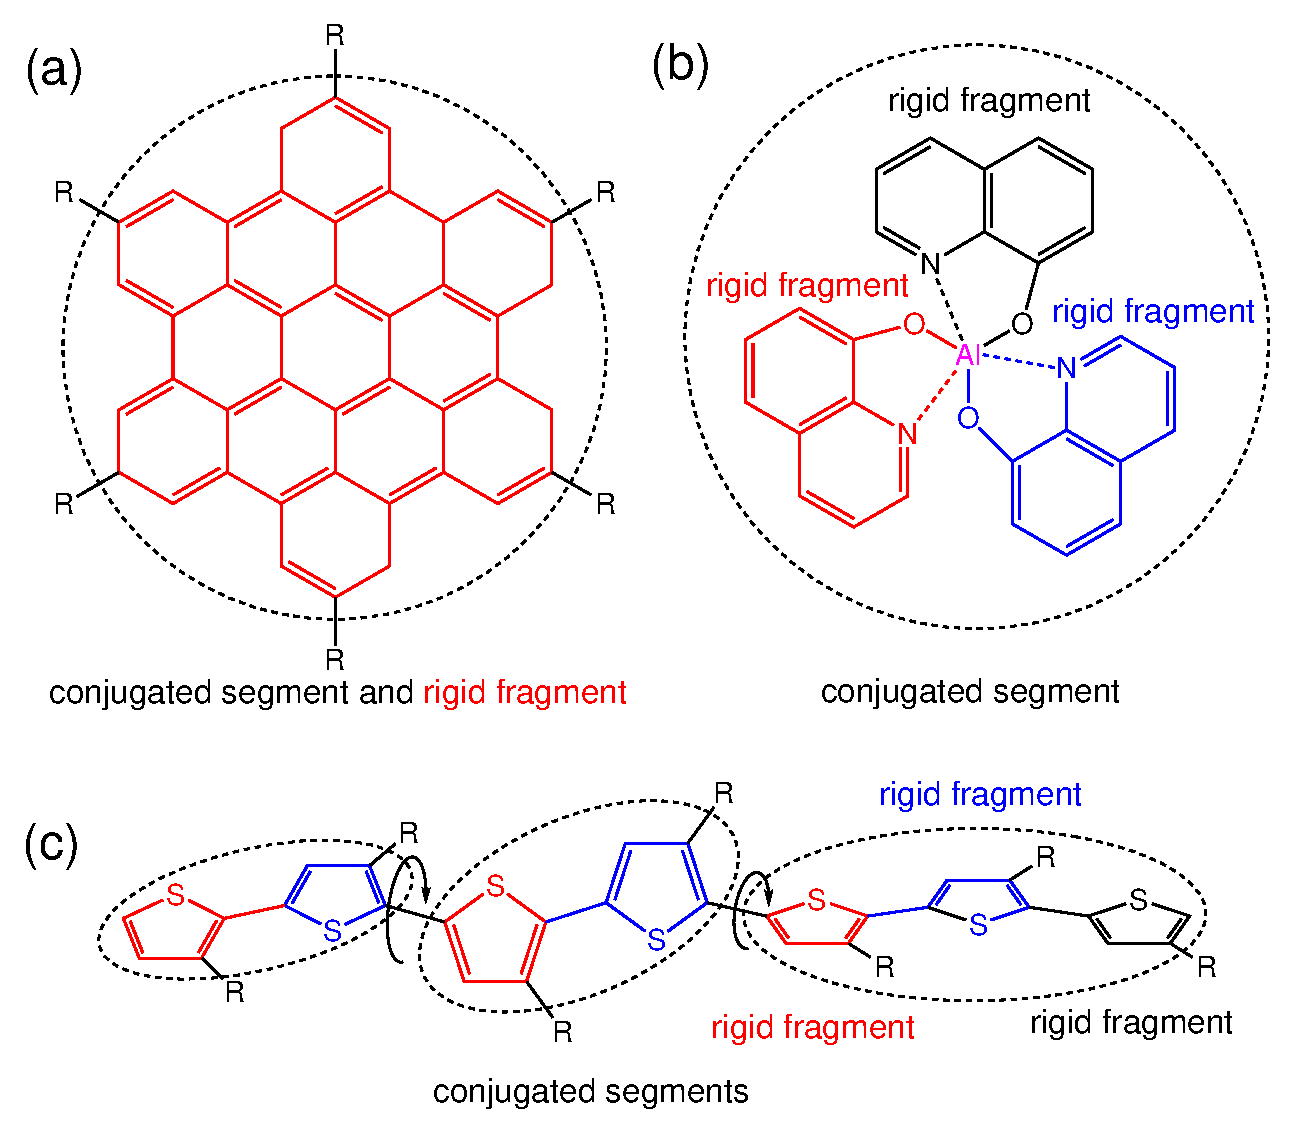
\includegraphics[width=\linewidth]{fig/conjugated_segment/fragment_segment}
\caption{\footnotesize The concept of conjugated segments and rigid fragments. Dashed lines indicate conjugated segments while colors denote rigid fragments. (a) Hexabenzocoronene: the $\pi$-conjugated system is both a rigid fragment and a conjugated segment. (b) \Alq: the Al atom and each ligand are rigid fragments while the whole molecule is a conjugated segment. (c) Polythiophene: each repeat unit is a rigid fragment. A conjugated segment consists of one or more rigid fragments. One molecule can have several conjugated segments.}
\label{fig:segment}
\end{wrapfigure}

With the morphology at hand, the next step is partitioning the system on hopping sites, or conjugated segments, and calculating charge transfer rates between them. Physically intuitive arguments can be used for the partitioning,  which reflects the localization of the wave function of a charge. For most organic semiconductors, the molecular architecture includes relatively rigid, planar $\pi$-conjugated systems, which we will refer to as rigid fragments. A conjugated segment can contain one or more of such rigid fragments, which are linked by bonded degrees of freedom. The dynamics of these degrees of freedom evolves on timescales much slower than the frequency of the internal promoting mode. In some cases, e.g. glasses, it can be `frozen' due to non-bonded interactions with the surrounding molecules.

To illustrate the concept of conjugated segments and rigid fragments, three representative molecular architectures are shown in \fig{segment}. The first one is a typical discotic liquid crystal, hexabenzocoronene. It consists of a conjugated core to which side chains are attached to aid self-assembly and solution processing. In this case the orbitals localized on side chains do not participate in charge transport and the conjugated $\pi$-system is both, a rigid fragment and a conjugated segment. 
%
In \Alq, a metal-coordinated compound, a charge carrier is delocalized over all three ligands. Hence, the whole molecule is one conjugated segment. Individual ligands are relatively rigid, while energies of the order of $k_\text{B}T$ are sufficient to reorient them with respect to each other. Thus the Al atom and the three ligands are rigid fragments.
%
In the case of a conjugated polymer, one molecule can consist of several conjugated segments, while each backbone repeat unit is a rigid fragment. Since the conjugation along the backbone can be broken due to large out-of-plane twists between two repeat units, an empirical criterion, based on the dihedral angle, can be used to partition the backbone on conjugated segments~\cite{ruehle_multiscale_2010}. However, such intuitive partitioning is, to some extent, arbitrary and shall be validated by other methods~\cite{vukmirovi_charge_2008,vukmirovi_charge_2009,mcmahon_ad_2009}. 

After partitioning, an additional step is often required to remove bond length fluctuations introduced by molecular dynamics simulations, since they are already integrated out in the derivation of the rate expression. This is achieved by substituting respective molecular fragments with  rigid, planar $\pi$-systems optimized using first-principles methods. Centers of mass and gyration tensors are used to align rigid fragments, though a custom definition of local axes is also possible. Such a procedure also minimizes discrepancies between the force-field and first-principles-based ground state geometries of conjugated segments, which might be important for calculations of electronic couplings, reorganization energies, and intramolecular driving forces. 

Finally, a list of neighboring conjugated segments is constructed. Two segments are added to this list if the distance between centers of mass of {\em any} their rigid fragments is below a certain cutoff. This allows neighbors to be selected on a criterion of minimum distance of approach rather than center of mass distance, which is useful for molecules with anisotropic shapes.


In addition to coordinates and atom tyoes, the code needs to know how the system is partitioned on  \hyperref[sec:conjugated_segments]{conjugated segments}, which represent localized electronic states available for mobile carriers. 


\section{Neighbor list}
\label{sec:neighborlist}

A list of neigboring molecules (neighbor list) containes all pairs of molecules for which rates (coupling elements, reorganization energies, and site energy differences are evaluated).

Two segments are added to this list if the distance between centers of mass of any of their rigid fragments is below
a certain cutoff. This allows neighbors to be selected on a criterion of minimum distance of approach rather than center of
mass distance, which is useful for molecules with anisotropic shapes.

The neighbor list can be generated from the atomistic trajectory by using the \calc{neighborlist} \calculator. This calculator requires a cutoff, which can be specified in the \xmloptions file. The list is saved to the \sqlstate file:

{\small \ctprun \opt \xmloptions  \seg  \xmlsegments \sql  \sqlstate \exe  \calc{neighborlist} }

\section{Reorganization energy}
\label{sec:reorganization}

The reorganization energy\index{reorganization energy} $\lambda_{ij}$ takes into account the change in  nuclear (and dielectric) degrees of freedom as the charge moves from donor $i$ to acceptor $j$. It has two contributions: intramolecular, $\lambda^\text{int}_{ij}$, which is due to reorganization of nuclear coordinates of the two molecules forming the charge transfer complex, and intermolecular (outersphere), $\lambda^\text{out}_{ij}$, which is due to the relaxation of the nuclear coordinates of the environment. In what follows we discuss how these contributions can be calculated.

\subsection{Intramolecular reorganization energy}
\label{sec:eintramolecular}
\index{reorganization energy!intramolecular}
If intramolecular vibrational modes of the two molecules are treated classically, the rearrangement of their nuclear coordinates after charge transfer results in the dissipation of the internal reorganization energy, $\lambda_{ij}^\text{int}$. It can be computed from four points on the potential energy surfaces (PES) of both molecules in neutral and charged states, as indicated in \fig{parabolas}. 

\begin{figure}
   \centering
   \includegraphics[width=0.6\linewidth]{fig/reorganization_energy/monomer_parabolas}
    \caption{Potential energy surfaces of (a) donor and (b) acceptor in charged and neutral states. After the change of the charge state both molecules relax their nuclear coordinates. If all vibrational modes are treated classically, the total internal reorganization energy and the internal energy difference of the electron transfer reaction are $\lambda_{ij}^\text{int} = \lambda_{i}^{cn} + \lambda_{j}^{nc}$ and $\Delta E_{ij}^\text{int} =  \Delta U_i - \Delta U_j$, respectively.}
   \label{fig:parabolas}
\end{figure}


Adding the contributions due to discharging of molecule $i$ and charging of molecule $j$ yields~\cite{bredas_charge-transfer_2004}
\begin{equation}
\lambda_{ij}^\text{int} =\lambda_{i}^{cn}+\lambda_{j}^{nc}=U_{i}^{nC}-U_{i}^{nN}+U_{j}^{cN}-U_{j}^{cC}\,.
\label{equ:lambdas}
\end{equation}
Here $U_{i}^{nC}$ is the internal energy of the neutral molecule $i$ in the geometry of its charged state (small $n$ denotes the state and capital $C$ the geometry). Similarly, $U_{j}^{cN}$ is the energy of the charged molecule $j$ in  the geometry of its neutral state.
%If the PES of neutral and charged states are different for the same molecule, that is  $\lambda^{cn}_i \neq \lambda^{nc}_i$, the rate for the bimolecular charge transfer is no longer a simple sum. If, as before, both modes are treated classically, the rate is an integral over the charge detachment and attachment spectrum of molecules $i$ and $j$~\cite{kakitani_comprehensive_1987}. For most systems, however, the reorganization energies for charging or discharging of the same molecule do not deviate by more than a few percent and the rate is given by~\equ{marcus}.
%
Note that the PES of the donor and acceptor are not identical for chemically different compounds or for conformers of the same molecule. In this case $\lambda_{i}^{cn} \ne \lambda_{j}^{cn}$ and  $\lambda_{i}^{nc} \ne \lambda_{j}^{nc}$. Thus $\lambda_{ij}^\text{int}$ is a property of the charge transfer complex, and not of a single molecule.

Intramolecular reorganization energies for discharging ($\lambda^{cn}$) and charging ($\lambda^{nc}$) of a molecule are provided in the \xmlsegments file and are written to the \sqlstate file by the \ctpmap program. 

\subsection{Outersphere reorganization energy}
\index{reorganization energy!outersphere}
\label{sec:eoutersphere}
During the charge transfer reaction, also the molecules outside the charge transfer complex reorient and polarize in order to adjust for changes in electric potential, resulting in the outersphere contribution to the reorganization energy. $\lambda_{ij}^\text{out}$ is particularly important if charge transfer occurs in a polarizable environment. Assuming that charge transfer is much slower than electronic polarization but much faster than nuclear rearrangement of the environment, $\lambda_{ij}^\text{out}$ can be calculated from the electric displacement fields created by the charge transfer complex~\cite{may_charge_2003}
\begin{equation}
\lambda_{ij}^\text{out}=
\frac{c_p}{2\epsilon_0}\int_{V^\text{out}}d V
\left[ \vec{D}_I(\vec{r}) - \vec{D}_F(\vec{r}) \right]^2\,,
\label{equ:lambda_outer1}
\end{equation}
where $\epsilon_0$ is the the permittivity of free space, $\vec{D}_{I,F}(\vec{r})$ are the electric displacement fields created by the charge transfer complex in the initial (charge on molecule $i$) and final (charge transferred to molecule $j$) states,  $V^\text{out}$ is the volume outside the complex, and $c_p=\frac{1}{\epsilon_\text{opt}}-\frac{1}{\epsilon_\text{s}}$ is the Pekar factor, which is determined by the low ($\epsilon_\text{s}$) and high ($\epsilon_\text{opt}$) frequency dielectric permittivities.

\Equ{lambda_outer1} can be simplified by assuming spherically symmetric charge distributions on molecules $i$ and $j$ with total charge $e$. Integration over the volume $V^\text{out}$ outside of the two spheres of radii $R_i$ and $R_j$ centered on molecules $i$ and $j$ leads to the classical Marcus expression for the outersphere reorganization energy
\begin{equation}
\lambda_{ij}^\text{out}=\frac{c_{p}e^2}{4\pi\epsilon_0}\left(\frac{1}{2 R_i}+\frac{1}{2 R_j}-\frac{1}{r_{ij}} \right)\,,
\label{equ:lambda_outer2}
\end{equation}
where $r_{ij}$ is the molecular separation.  While \equ{lambda_outer2} captures the main physics, e.g. predicts smaller outer-sphere reorganization energies (higher rates) for molecules at smaller separations, it often cannot provide quantitative estimates, since charge distributions are rarely spherically symmetric. 

Alternatively, the displacement fields can be constructed using the atomic partial charges. The difference of the displacement fields at the position of an atom $b_k$ outside the charge transfer complex (molecule $k \ne i,j$)  can be expressed as
\begin{eqnarray}
\label{equ:disp_atom}
\vec{D}_I(\vec{r}_{b_k}) - \vec{D}_F(\vec{r}_{b_k})  = 
\sum_{a_i} \frac{q_{a_i}^c - q_{a_i}^n}{4\pi } \frac{ (\vec{r}_{b_k} - \vec{r}_{a_i} ) }
                                            {|\vec{r}_{b_k}-\vec{r}_{a_i}|^3}+
\sum_{a_j} \frac{q_{a_j}^n - q_{a_j}^c}{4\pi } \frac{ (\vec{r}_{b_k}-\vec{r}_{a_j} ) } 
                                            {|\vec{r}_{b_k}-\vec{r}_{a_j}|^3}\,,
%\nonumber
\end{eqnarray}
where $q^n_{a_i}$ ($q^c_{a_i}$) is the partial charge of atom $a$ of the neutral (charged) molecule $i$ in vacuum. The partial charges of neutral and charged molecules are obtained by fitting their values to reproduce the electrostatic potential of a single molecule (charged or neutral) in vacuum. 
%
Assuming a uniform density of atoms, the integration in~\equ{lambda_outer1} can be rewritten as a density-weighted sum over all atoms excluding those of the charge transfer complex.

The remaining unknown needed to calculate $\lambda_{ij}^\text{out}$ is the Pekar factor\index{Pekar factor}, $c_p$. In polar solvents $\epsilon_\text{s}\gg\epsilon_\text{opt}\sim 1$ and $c_p$ is of the order of 1. In most organic semiconductors, however, molecular orientations are fixed and therefore the low frequency dielectric permittivity is of the same order of magnitude as $\epsilon_\text{opt}$. Hence, $c_p$ is small and its value is very sensitive to differences in the permittivities. 


Outersphere reorganization energies for all pairs of molecules in the \slink{neighborlist}{neighbor list} can be computed from the atomistic trajectory by using the \calc{eoutersphere} \calculator. 

Two methods can be used to compute $\lambda_{ij}^\text{out}$. The first method uses the atomistic partial charges of neutral and charged molecules from files specified in \xmlsegments and \equ{lambda_outer1}. The Pekar factor $c_p$ and a cutoff radius  based on molecular centers of mass have to be specified in the \xmloptions file. 

If this method is computationally prohibitive, $\lambda_{ij}^\text{out}$ can be computed using \equ{lambda_outer2}, which assumes spherical charge distributions on the molecules. In this case the radii of these spheres are specified in \xmlsegments, while the Pekar factor $c_p$ is given in the \xmloptions file and no cutoff radius is needed. 

The outer sphere reorganization energies are saved to the \sqlstate file:

{\small \ctprun \opt \xmloptions  \seg  \xmlsegments \sql  \sqlstate \exe  \calc{eoutersphere}}

\section{Site energies}
\label{sec:site_energies}
A charge transfer reaction between molecules $i$ and $j$ is driven by the site energy\index{site energy} difference, $\Delta E_{ij} = E_i - E_j$. Since the  transfer rate, $\omega_{ij}$, depends exponentially on $\Delta E_{ij}$ (see~\equ{marcus}) it is important to compute its distribution as accurately as possible.  The total site energy difference has contributions due to \slink{sec:ext_field}{externally applied electric field}, \slink{sec:ecoulomb}{electrostatic interactions}, polarization effects, and \slink{sec:internal_energy}{internal energy} differences. In what follows we discuss how to estimate these contributions by making use of first-principles calculations and polarizable force-fields.

\subsection{Externally applied electric field}
\label{sec:ext_field}
The contribution to the total site energy\index{site energy!external field} difference due to an external electric field $\vec{F}$ is given by $\Delta E_{ij}^\text{ext} = q {\vec{F} \cdot \vec{r}_{ij}}$, where $q=\pm e$ is the charge and $\vec{r}_{ij} = \vec{r}_i  - \vec{r}_j $ is a vector connecting molecules $i$ and $j$. For typical distances between small molecules, which are of the order  of $1\,\unit{nm}$, and moderate fields of $F<10^8\,\unit{V/m}$ this term is always smaller than $0.1\, \unit{eV}$.

\subsection{Internal energy}
\label{sec:internal_energy}

The contribution to the site energy difference due to different internal energies\index{site energy!internal} (see \fig{parabolas}) can be written as
\begin{equation}
 \Delta E_{ij}^\text{int}=
\Delta U_i - \Delta U_j = \left( U_{i}^{cC}-U_{i}^{nN}\right) - \left( U_{j}^{cC}-U_{j}^{nN}\right) \, ,
\label{equ:conformational}
\end{equation}
where $U_{i}^{cC(nN)}$ is the total energy of molecule $i$ in the charged (neutral) state and geometry.  $\Delta U_{i}$ corresponds to the adiabatic ionization potential (or electron affinity) of molecule $i$, as shown in~\fig{parabolas}. For one-component systems and negligible conformational changes $ \Delta E_{ij}^\text{int}=0$, while it is significant for donor-acceptor systems. 

Internal energies determined using quantum-chemistry need to be specified in \xmlcsg. The values are written to the \sqlstate using the calculator \calc{einternal} (see also \slink{sec:eintramolecular}{intramolecular reorganization energy}):
\votcacommand{Internal energies}{\cmdeint}

\section{Electronic coupling elements}
\label{sec:transfer_integrals}

The electronic transfer integral\index{electronic coupling} element $J_{ij}$ entering the Marcus rates in \equ{marcus} is defined as
\begin{equation}
   J_{ij} = \left\langle \phi^i \left\vert \hat{H} \right\vert \phi^j \right\rangle ,
\label{equ:TI}
\end{equation}
where $\phi^i$ and $\phi^j$ are diabatic wavefunctions, localized on molecule $i$ and $j$ respectively, participating in the charge transfer, and $\hat{H}$ is the Hamiltonian of the formed dimer. Within the frozen-core approximation, the usual choice for the diabatic wavefunctions $\phi^i$  is the highest occupied molecular orbital (HOMO) in case of hole transport, and the lowest unoccupied molecular orbital (LUMO) in the case of electron transfer, while $\hat{H}$ is an effective single particle Hamiltonian, e.g. Fock or Kohn-Sham operator of the dimer. As such, $J_{ij}$ is a measure of the strength of the electronic coupling of the frontier orbitals of monomers mediated by the dimer interactions. Intrinsically, the transfer integral is very sensitive to the molecular arrangement, i.e. the distance and the mutual orientation of the molecules participating in charge transport. Since this arrangement can also be significantly influenced by
static and/or dynamic disorder~\cite{hutchison_hopping_2005,kirkpatrick_columnar_2008,troisi_charge_2009,vehoff_charge_2010-1,vehoff_charge_2010-2},
it is essential to calculate $J_{ij}$ explicitly for each hopping pair within a realistic morphology. Considering that the number of dimers for which \equ{TI} has to be evaluated is proportional to the number of molecules times their coordination number, computationally efficient and at the same time quantitatively reliable schemes are required.

In general, information about three objects is needed: the two monomer wave functions $\phi^i$ and $\phi^j$, and the dimer interaction Hamiltonian $\hat{H}$.  

\subsection{Semi-empirical methods}
\label{sec:moo}

\newcommand{\moo}{MOO\xspace}
\index{electronic coupling!ZINDO}

An approximate method based on Zerner's Independent Neglect of Differential Overlap (ZINDO) has been described in Ref.~\cite{kirkpatrick_approximate_2008}. This semiempirical method is substantially faster than first-principles approaches, since it avoids the self-consistent calculations on each individual monomer and dimer. This allows to construct the matrix elements of the ZINDO Hamiltonian of the dimer from the weighted overlap of molecular orbitals of the two monomers. Together with the introduction of rigid segments, only a single self-consistent calculation on one isolated conjugated segment is required. All relevant molecular overlaps can then be constructed from the obtained molecular orbitals. This Molecular Orbital Overlap (MOO) method has been applied successfully to study charge transport, for instance, in discotic liquid crystals~\cite{kirkpatrick_columnar_2008,marcon_understanding_2009,feng_towards_2009},
polymers~\cite{ruehle_multiscale_2010}, or partially disordered organic crystals~\cite{vehoff_charge_2010-1,vehoff_charge_2010-2,vehoff_charge_2010}.

The main advantage of the molecular orbital overlap \moo library is {\em fast} evaluation of electronic coupling elements. A detailed description of the method is provided in ref.~\cite{kirkpatrick_approximate_2008}. Please site this paper if you are using the method. Note that \moo is based on the semi-empirical ZINDO Hamiltonian and therefore has limited applicability. The general advice is to first compare the accuracy of the \moo method to the DFT-based calculations. 

\moo can be used both in a sandalone mode and as a \calculator of the \votcactp. \moo constructs the Fock operator of a dimer from the  molecular orbitals of monomers by translating and rotating the orbitals and therefore requires the optimized geometry of the molecule and the projection coefficients of the molecular on atomic orbitals. 


\subsubsection{Standalone mode}
For a standalone mode program \overlap is provided 
\begin{verbatim}
 moo_overlap --conjseg benzene.xml --pos1 benzene1.pos --pos2 benzene2.pos
\end{verbatim}
Its input requires a description of two conjugated segments (\texttt{benzene.xml}, positions and orientations of the molecules and the files with molecular coordinates and orbitals. The structure of the files is shown in listings \ref{list:benzene_xml} and  \ref{list:benzene_pos}.
\vskip 0.1cm
\lstinputlisting[
  language=XML,
  label=list:benzene_xml,
  stringstyle=\ttfamily\footnotesize,
  showstringspaces=false,
  caption={\small \texttt{benzene.xml} file with the description of the benzene molecule, which is also a single conjugated segment and a rigid fragment.}] {./programs/benzene.xml}

\vskip 0.1cm

\lstinputlisting[
  language=XML,
  label=list:benzene_pos, 
  stringstyle=\ttfamily\footnotesize,
  showstringspaces=false,
  caption={\small \texttt{benzene1.pos} file which describes the position and orientation of the molecule. The name of the molecule is followed by three coordinates (relative to the center of mass of the supplied \texttt{xyz} file and then by nine elements of the rotation matrix $a_{ij} = e_i e^\text{mol}_j $. The reference coordinate frame is determined from the provided \texttt{xyz} file.}] {./fig/moo/moo_overlap/benzene1.pos}


\subsubsection{Calculator of \votcactp}
Semi-empirical method of evaluation of electronic couplings in a morphology is provided by the \integrals \calculator. In addition to definitions of conjugated segments, atomistic trajectory, and state file, the program needs coordinates and orbitals of conjugated segments. Coordinates are stored in \xyz files with four columns, first being the atom type and the next three atom coordinates. This is a standard \texttt{xyz} format without a header. Note that the atom order in \xyz files can be different from that of the mapping files. The correspondence between the two is established in the file which defines conjugated segments.

\subsection{Density-functional methods}
\label{sec:dft}
\index{electronic coupling!DFT}
While the use of the semiempirical ZINDO method provides an efficient on-the-fly technique to determine electronic coupling elements, it is not generally applicable to all systems. For instance, its predictive capacity with regards to atomic composition and localization behavior of orbitals within more complex structures is reduced. Moreover, transition- or semi-metals are often not even parametrized. In this case, {\it ab-initio} based approaches, e.g., density-functional theory can remedy the situation~\cite{huang_intermolecular_2004,huang_validation_2005,valeev_effect_2006,yin_balanced_2006,yang_theoretical_2007,baumeier_density-functional_2010}. Within the dimer projection method described in detail in Ref.~\cite{baumeier_density-functional_2010}, explicit quantum-chemical calculations are required for every molecule and every hopping pair in the morphology. As a consequence, this procedure is significantly more computationally demanding. The code currently contains scripts which support evaluation of transfer integrals from quantum-chemical calculations performed with the \gaussian and \turbomole packages.

Apart from semi-empirical methods, we also provide interfaces for a DFT-based evaluation of electronic coupling elements. The interfacing procedure consists of three main steps: generation of directory structures containing input coordinates for monomers and dimers, performing the actual quantum-chemical calculations and calculating the transfer integrals using the DIPRO method, and finally reading the output into VOTCA\_CT.

\subsubsection{Generation of directory structure and input coordinates}
First, hopping sites and a neighbor list need to be generated from the atomistic topology and trajectory. Rigid fragments are resubstituted into the molecular geometries and the neighbor list is defined based on a cutoff distance between such fragments. This can be achieved by running, e.g.  
\begin{verbatim}
ctp_map [required options] --db state.db --nframes 1 --first-frame 1
\end{verbatim}
to generate a state file is for first frame of the trajectory. Then a neighbor list can be determined from the cutoff defined in {\tt main.xml} (see \ref{list:neighborcut_xml}).
\lstinputlisting[
  language=XML,
  label=list:neighborcut_xml,
  stringstyle=\ttfamily\footnotesize,
  showstringspaces=false,
  caption={\small Definition of neighborlist cutoff in {\tt main.xml}}.] {./programs/neighborcut.xml}
by calling
\begin{verbatim}
ctp_run --opt main.xml --s segments.xml --db state.db --exec neighborlist
\end{verbatim}
and from that the full file and directory structure needed by {\tt ctp\_dipro} is written by 
\begin{verbatim}
ctp_run --opt main.xml --s segments.xml --db state.db --exec pairdump
\end{verbatim}
This requires the specification of the content of listing \ref{list:pairdump_xml} in {\tt main.xml}.
\lstinputlisting[
  language=XML,
  label=list:pairdump_xml,
  stringstyle=\ttfamily\footnotesize,
  showstringspaces=false,
  caption={\small Block of pairdump options required in {\tt main.xml} for generating the directory structure and coordinate files for {\tt ctp\_dipro}.}] {./programs/pairdump.xml}
After this, the following directories and files have been created:
\begin{verbatim}
|----frame1/
| |----mol_1/
| | |----mol_1.xyz
| | [...]
| |----pair_1_2/
| | |----dim/
| | | |----pair_1_2.xyz
| | [...]
\end{verbatim}

\subsubsection{Calculating the transfer integrals}
Before starting the quantum-chemical calculations with either {\tt Gaussian} or {\tt Turbomole}, make sure that the respective environments for these programs are set. 

First, for each molecule a converged electronic structure calculatiom has to be performed by running 
\begin{verbatim}
ctp_dipro --monomer QCP [METHOD]

QCP:   G for Gaussian09
       T for Turbomole

METHOD: func/basis (optional)
        overrides default functional/basisset combination
        defaults: pbepbe/6-311G** Gaussian09
                  pbe/def-TZVP    Turbomole
\end{verbatim}
in each {\tt mol\_*} directory. If no method is specified, {\tt ctp\_dipro} defaults to running a DFT calculation with the PBE functional and a 6-311G** basis set in {\tt Gaussian} and def-TZVP in {\tt Turbomole}. Note that {\tt OpenBabel} needs to be installed is {\tt Turbomole} is used. It is recommended to perform these calculations in batch mode on some kind of cluster system. Since it can eventually happen that files are not written back correctly, one should check if all files that are needed for the pair runs are present by executing in the {\tt frame*} directory
\begin{verbatim}
ctp_dipro --check N M QCP

N:   First monomer to test
M:   Last monomer to test
QCP: G/T 
\end{verbatim}
A list of incomplete monomer calculations is written to file {\tt TROUBLE.mol}. If this is empty, one can proceed with running the pair calculations. For any directory {\tt pair\_A\_B}, the completed monomer calculations from the previous step have to be present in subdirectories {\tt mol\_A} and {\tt mol\_B}, e.g.
\begin{verbatim}
| | [...]
| |----pair_1_2/
| | |----molA/
| | |----molB/
| | |----dim/
| | | |----pair_1_2.xyz
| | [...]
\end{verbatim}
These subdirectories can be either copies or symbolic links, however, the most practical realization depends on the specifics of execute machine (e.g. local or network, hard disc etc.) so that these are not created automatically! Once these are created by the user, the transfer integral for the pair can be calculated by running {\tt ctp\_dipro --dimer} in the {\tt pair\_A\_B/dim} directory:
 \begin{verbatim}
ctp_dipro --dimer QCP [METHOD]

QCP:   G for Gaussian09
       T for Turbomole

METHOD: func/basis (optional)
        overrides default functional/basisset combination
        defaults: pbepbe/6-311G** Gaussian09
                  pbe/def-TZVP    Turbomole
\end{verbatim}
This command automatically generates a dimer input guess from the converged monomer orbitals, detects (pseudo-)degeneracies of HOMO or LUMO and calculates the required transfer integrals. As a result of the run, a file {\tt pair\_A\_B/TI.xml} as shown in listing \ref{list:TI_xml} is created (needs proper example).
\lstinputlisting[
  language=XML,
  label=list:TI_xml,
  stringstyle=\ttfamily\footnotesize,
  showstringspaces=false,
  caption={\small Example {\tt TI.xml} file created as the output of a DIPRO calculation. Due to slightly different implementations, the orbitals indices refer to monomer indices in a {\tt Gaussian} run but to indices in the merged dimer guess in a {\tt Turbomole} run.}] {./programs/TI.xml}

\subsubsection{Writing transfer integrals to state file}
After performing all transfer integral calculations, the resulting output files {\tt pair\_A\_B/TI.xml} have to be collected in the folder {\tt transfer\_integrals} as {\tt transfer\_integrals/pair\_A\_B.xml}. Then the transfer integrals are written into the state file using:
\begin{verbatim}
ctp_dipro --write TYPE ID FILE

TYPE:   e    - electrons
        h    - holes
        edeg - (pseudo-)degenerate electrons (Boltzmann-weighted)
        hdeg - (pseudo-)degenerate holes (Boltzmann-weighted)
ID:     Number of frame
FILE:   Name of state file 
\end{verbatim}
During the run, some sanity checks are performed, i.e., whether all transfer integrals are calculated, and whether a pair that is written exists in the state file. If there is an error, the tool aborts.


\section{Charge transfer rate}

Charge transfer rates can be postulated based on intuitive physical considerations, as it is done in the Gaussian disorder models~\cite{walker_electrical_2002,baessler_charge_1993,borsenberger_charge_1991,pasveer_unified_2005}. Alternatively, charge transfer theories can be used to evaluate rates from quantum chemical calculations~\cite{bredas_molecular_2009,coropceanu_charge_2007,bredas_charge-transfer_2004,nelson_modeling_2009,baumeier_density-functional_2010,kirkpatrick_approximate_2008}. In spite of being significantly more computationally demanding, the latter approach allows to link the chemical and electronic structure, as well as the morphology, to charge dynamics.

\subsection{Classical charge transfer rate}
The high temperature limit of classical charge transfer  theory~\cite{marcus_electron_1993,hutchison_hopping_2005} is often used as a trade-off between theoretical rigor and computational complexity. It captures key parameters which influence charge transport while at the same time providing an analytical expression for the rate. Within this limit, the transfer rate for a charge to hop from a site $i$ to a site $j$ reads
%
\begin{equation}
\omega_{ij}  = \frac{2 \pi}{\hbar}  \frac{ J_{ij}^2 }{\sqrt{ 4 \pi \lambda_{ij} k_\text{B}T}} \exp \left[
-\frac{\left(\Delta E_{ij}-\lambda_{ij}\right)^2}{4 \lambda_{ij}
k_\text{B} T} \right],
\label{equ:marcus}
\end{equation}
%
where $T$ is the temperature, $\lambda_{ij} = \lambda_{ij}^\text{int} + \lambda_{ij}^\text{out}$ is the reorganization energy, which is a sum of intra- and inter-molecular (outer-sphere) contributions, $\Delta E_{ij}$ is the site-energy difference, or driving force, and $J_{ij}$ is the electronic coupling element, or transfer integral~\cite{note_marcus}. A more general, quantum-classical expression for a bimolecular multi-channel rate is derived in the Supporting Information.

All the ingredients entering \equ{marcus} can be calculated using electronic structure techniques, classical simulation methods, or their combination. With the rates at hand, one can study charge transport by solving the differential (master) equation, e.g. by using the kinetic Monte Carlo method which is capable of simulating charge dynamics of non-steady-state systems.

\subsection{Semi-classical bimolecular rate}
The main assumptions in eq.~(\ref{equ:marcus}) are non-adiabaticity (small electronic coupling and  charge transfer between two diabatic, non-interacting states), and harmonic promoting modes, which are treated classically. At ambient conditions, however, the intramolecular promoting mode, which roughly corresponds to C-C bond stretching, has a vibrational energy of $\hbar\omega \approx 0.2\, \unit{eV} \gg k_\text{B}T$ and should be treated quantum-mechanically. The outer-sphere (slow) mode has much lower vibrational energy than the intramolecular promoting mode, and therefore can be treated classically. The weak interaction between molecules also implies that each molecule has its own, practically independent, set of quantum mechanical degrees of freedom.
A rate expression for the aforementioned situation is derived in the supporting information. Numerical estimates show that if  $\lambda_{ij}^\text{int} \approx \lambda_{ij}^\text{out}$ and $|\Delta E_{ij}| \ll \lambda_{ij}^\text{out}$ the rates are similar to those of ~\equ{marcus}. In general, there is no robust method to compute $\lambda_{ij}^\text{out}$~\cite{hoffman_reorganization_1996} and  both reorganization energies are often assumed to be of the same order of magnitude. In this case the second condition also holds, unless there are large differences in electron affinities or ionization potentials of neighboring molecules, e.g. in donor-acceptor blends.
\section{Master equation}
\label{sec:kmc}
\index{kinetic Monte Carlo}
Having determined the list of conjugated segments (hopping sites) and charge transfer rates between them, the next task is to solve the master equation which describes the time evolution of the system
%
\begin{equation}
\label{equ:master}
\frac{\partial P_\alpha}{\partial t} = \sum_{\beta} P_\beta \Omega_{\beta \alpha} - 
\sum_{\beta} P_\alpha \Omega_{\alpha \beta},
\end{equation}
%
where $P_\alpha$ is the probability of the system to be in a state $\alpha$ at time $t$ and $\Omega_{\alpha \beta}$ is the transition rate from state $\alpha$ to state $\beta$. A state $\alpha$ is specified by a set of site occupations, $\left\{ \alpha_i \right\}$, where $\alpha_i = 1 (0)$ for an occupied (unoccupied) site $i$, and the matrix $\hat{\Omega}$ can be constructed from rates $\omega_{ij}$.

The solution of \equ{master} is be obtained by using kinetic Monte Carlo (KMC) methods. KMC explicitly simulates the dynamics of charge carriers by constructing a Markov chain in state space and can find both stationary and transient solutions of the master equation. The main advantage of KMC is that only states with a direct link to the current state need to be considered at each step. Since these can be constructed solely from current site occupations, extensions to multiple charge carriers (without the mean-field approximation), site-occupation dependent rates (needed for the explicit treatment of Coulomb interactions), and different types of interacting particles and processes, are straightforward. To optimize memory usage and efficiency, a combination of the variable step size method~\cite{bortz_new_1975} and the first reaction method is implemented.

To obtain the dynamics of charges using KMC, the program \kmcrun executes a specific \calculator after reading its options (charge carrier type, runtime, numer of carriers etc.) from \xmloptions. 

\votcacommand{KMC for a single carrier in periodic boundary conditions}{\cmdkmcsin}

\votcacommand{KMC for multiple carriers of the same type in periodic boundary conditions}{\cmdkmc}


%\subsection{Extrapolation to nondispersive mobilities}
\label{sec:nondispersive}
Predictions of charge-carrier mobilities in partially disordered semiconductors  rely on charge transport simulations in systems which are only several nanometers thick. As a result, simulated charge transport might be dispersive for materials with large energetic disorder~\cite{scher_anomalous_1975,borsenberger_role_1993} and simulated mobilities are system-size dependent. In time-of-flight (TOF) experiments, however, a typical sample thickness is in the micrometer range and transport is often nondispersive. In order to link simulation and experiment, one needs to extract the nondispersive mobility from simulations of small systems, where charge transport is dispersive at room temperature.

Such extrapolation is possible if the temperature dependence of the nondispersive mobility is known in a wide temperature range. For example, one can use analytical results derived for one-dimensional models~\cite{derrida_velocity_1983,cordes_one-dimensional_2001,seki_electric_2001}. The mobility-temperature dependence can then be parametrized by simulating charge transport at elevated temperatures, for which transport is nondispersive even for small system sizes. This dependence can then be used to extrapolate to the nondispersive mobility at room temperature~\cite{lukyanov_extracting_2010}.

For \Alq, the charge carrier mobility of a periodic system of 512 molecules was shown to be more than three orders of magnitude higher than the nondispersive mobility of an infinitely large system~\cite{lukyanov_extracting_2010}. Furthermore, it was shown that the transition between the dispersive and nondispersive transport has a logarithmic dependence on the number of hopping sites $N$. Hence, a brute-force increase of the system size cannot resolve the problem for compounds with large energetic disorder $\sigma$, since $N$ increases exponentially with $\sigma^2$.
 


\section{Macroscopic observables}
\label{sec:analysis}%
Spatial distributions of charge and current densities can provide a better insight in the microscopic mechanisms of charge transport.
%
If $O$ is an observable which has a value $O_\alpha$ in a state $\alpha$, its ensemble average at time $t$ is a sum over all states weighted by the probability $P_\alpha$ to be in a state $\alpha$ at time $t$
%
\begin{equation}
\label{equ:ensemble}
\left< O \right> = \sum_{\alpha} O_\alpha P_\alpha.
\end{equation}
%
If $O$ does not explicitly depend on time, the time evolution of $\left< O \right>$ can be calculated as
\begin{equation}
\begin{split}
\frac{d \left< O \right>}{dt} = \sum_{ \alpha, \beta} 
      \left[ P_\beta \Omega_{\beta \alpha} - 
       P_\alpha \Omega_{\alpha \beta} \right] 
      O_\alpha %\\
 %     
      = \sum_{ \alpha, \beta} 
      P_\beta \Omega_{\beta \alpha}  
      \left[ O_\alpha - O_\beta \right] .
\end{split}
\end{equation}
%
If averages are obtained from KMC trajectories, $P_\alpha = s_\alpha / s$, where $s_\alpha$ is the number of Markov chains ending in the state $\alpha$ after time $t$, and $s$ is the total number of chains.

Alternatively, one can calculate time averages by analyzing a single Markov chain. If the total occupation time of the state $\alpha$ is $\tau_\alpha$ then
\begin{align}
\label{equ:time}
\overline{ O } 
= \frac{1}{\tau} \sum_{\alpha} O_\alpha \tau_\alpha \,,
\end{align}
where $\tau = \sum_{\alpha} \tau_\alpha$ is the total time used for time averaging.

For ergodic systems and sufficient sampling times, ensemble and time averages should give identical results. 
In many cases, the averaging procedure reflects a specific experimental technique. For example, an ensemble average over several KMC trajectories with different starting conditions corresponds to averaging over injected charge carriers in a time-of-flight experiment.  In what follows, we focus on the single charge carrier (low concentration of charges) case. 

\subsection{Charge density}
\label{sec:occupation}

For a specific type of particles, the microscopic charge density of a site $i$ is proportional to the occupation probability of the site, $p_i$
\begin{equation}
 \rho_i = e p_i / V_i\, ,
\end{equation}
where,  for an irregular lattice, the effective volume $V_i$ can be obtained from a Voronoi tessellation of space. For reasonably uniform lattices (uniform site densities) this volume is almost independent of the site and a constant volume per cite, $V_i = V/N$, can be assumed.  In the macroscopic limit, the charge density can be calculated using a smoothing kernel function, i.e. a distance-weighted average over multiple sites. Site occupations $p_i$ can be obtained from \equ{ensemble} or  \equ{time} by using the occupation of site $i$ in state $\alpha$ as an observable.

If the system is in thermodynamic equilibrium, that is without sources or sinks and without circular currents (and therefore no net flux) a condition, known as detailed balance, holds
%
\begin{equation}
\label{equ:detailed_balance}
  p_j \omega_{ji} = p_i \omega_{ij},
\end{equation}
%
It can be used to test whether the system is ergodic or not by correlating $\log p_i$ and the site energy $E_i$. Indeed, if $\lambda_{ij} = \lambda_{ji}$ the ratios of forward and backward rates are determined solely by the energetic disorder, $\omega_{ji} / \omega_{ij} = \exp(-\Delta E_{ij} / k_\text{B} T)$ (see \equ{marcus}).

\subsection{Current}
\label{sec:vaverage}
\index{current}
If the position of the charge, $\vec{r}$, is an observable, the time evolution of its average $\left<\vec{r}\right>$ is the total current in the system
\begin{equation}
 \vec{J} = e \left< \vec{v} \right> = e \frac{d \left< \vec{r}
   \right>} {dt} = e \sum_{i, j} p_{j} \omega_{ji} ( \vec{r}_i -
 \vec{r}_j ) .
\label{equ:current_def}
\end{equation}
Symmetrizing this expression we obtain
\begin{equation}
  \vec{J} = \frac{1}{2} e \sum_{i, j} \left( p_{j} 
  \omega_{ji} - p_{i} \omega_{ij} \right) \vec{r}_{ij} ,
 \label{equ:current}
\end{equation}
where $\vec{r}_{ij} = \vec{r}_{i} - \vec{r}_{j}$. Symmetrization ensures equal flux
splitting between neighboring sites and absence of local average fluxes in equilibrium. It allows to define a local current through site $i$ as\index{current!local}
\begin{equation}
  \vec{J_i} = \frac{1}{2} e \sum_{ j} \left( p_{j}  \omega_{ji} - p_{i} \omega_{ij} \right) \vec{r}_{ij} .
 \label{equ:site_current}
\end{equation}
A large value of the local current indicates that the site contributes considerably to the total current. A collection of such sites thus represents most favorable charge pathways~\cite{van_der_holst_modeling_2009}.

\subsection{Mobility and diffusion constant}
\label{sec:mobility}
\index{mobility}
For a single particle, e.g. a charge or an exciton, a zero-field mobility can be determined by studying particle diffusion in the absence of external fields. Using the particle displacement squared, $\Delta {\bm r}_i^2$, as an observable  we obtain
 \begin{equation}
\begin{split}
2d D_{\gamma \delta} =  \frac{d \left<  \Delta{r}_{i, \gamma} \Delta{r}_{i, \delta} \right>}{dt} 
= \sum_{\substack{i,j \\ i\ne j}} p_j\omega_{ji} 
 \left( \Delta r_{i,\gamma}\Delta r_{i,\delta} - \Delta r_{j,\gamma}\Delta r_{j,\delta} \right)  
= \sum_{\substack{i,j\\ i\ne j}} p_j \omega_{ji} \left( r_{i,\gamma} r_{i,\delta} - r_{j,\gamma} r_{j,\delta} \right) \, .
\end{split}
\label{equ:diffusion}
\end{equation}
Here $\vec{r}_i$ is the coordinate of the site $i$, $D_{\gamma \delta}$ is the diffusion tensor, $\gamma, \delta = x,y,z$, and $d=3$ is the system dimension. Using the Einstein relation, 
\begin{equation}
 D_{\gamma \delta} = k_\text{B}T \mu_{\gamma \delta} \, ,
\end{equation}
one can, in principle, obtain the zero-field mobility tensor $\mu_{\gamma \delta}$. \Equ{diffusion}, however, does not take into account the use of periodic boundary conditions when simulating charge dynamics. In this case, the simulated occupation probabilities can be compared to the solution of the Smoluchowski equation with periodic boundary conditions  (see the supporting information for details). 

Alternatively, one can directly analyze time-evolution of the KMC trajectory and obtain the diffusion tensor from a linear fit to the mean square displacement, $\overline{ \Delta{r}_{i, \gamma} \Delta{r}_{i, \delta}} = 2d D_{\gamma \delta} t$. 

The charge carrier mobility tensor, $\hat{\mu}$, for any value of the external field can be determined either from the average charge velocity defined in
\equ{current_def} 
\begin{equation}
%\begin{split}
 \langle \vec{v} \rangle =  \sum_{i,j}  p_j  \omega_{ji}  (\vec{r}_i - \vec{r}_j) = \hat{\mu} \vec{F} \, ,
%\end{split}
\end{equation}
or directly from the KMC trajectory. In the latter case the velocity is calculated from the unwrapped (if periodic boundary conditions are used) charge displacement vector divided by the total simulation time. Projecting this velocity on the direction of the field $\vec{F}$ yields the charge carrier mobility in this particular direction. In order to improve statistics, mobilities can be averaged over several KMC trajectories and MD snapshots.

\subsection{Spatial correlations of energetic disorder}
\label{sec:ecorrelation}

Long-range, e.g. electrostatic and polarization, interactions often result in spatially correlated disorder~\cite{dunlap_charge-dipole_1996}, which affects the onset of the mobility-field (Poole-Frenkel) dependence~\cite{derrida_velocity_1983,novikov_essential_1998,nagata_atomistic_2008}.    

To quantify the degree of correlation, one can calculate the spatial correlation function of $E_i$ and $E_j$ at a distance $r_{ij}$
\begin{equation}
\label{equ:cf}
C(r_{ij}) = \frac{  \langle \left( E_i-\langle E\rangle \right)
                   \left( E_j-\langle E\rangle \right)\rangle}
                   {\langle\left( E_i -\langle E\rangle \right)^2\rangle},
\end{equation}
where $\langle E\rangle$ is the average site energy. $C(r_{ij})$ is zero if $E_i$ and $E_j$ are uncorrelated and $1$ if they are fully correlated. For a system of randomly oriented point dipoles, the correlation function decays as $1/r$ at large distances~\cite{novikov_cluster_1995}.

For systems with spatial correlations, variations in site energy differences, $\Delta E_{ij}$, of pairs of molecules from the neighbor list are smaller than variations in site energies, $E_i$, of all individual molecules. Since only neighbor list pairs affect transport, the distribution of $\Delta E_{ij}$ rather than that of individual site energies, $E_i$, should be used to characterize energetic disorder.

\chapter{Input and output files}
\label{sec:mapping}

\xml-based input files specify atomistic topology, coarse-grained topology, and define conjugated segments. In addition, practically every \calculator requires options provided in a separate \xml file.

\section{Atomistic topology}
\label{sec:atomistic}

If you are using \gromacs for generating atomistic configurations, it is possible to directly use the topology file provided by \gromacs (\texttt{topology.tpr}). In this case the \gromacs residue and atom names should be used to specify the \slink{mapping}{coarse-grained topology} and \slink{xmlsegments}{conjugated segments}. 

A custom topology can also be defined using an \xml file. Moreover, it s possible to partially overwrite the information provided in, for example, \gromacs topology file. We will illustrate how to create a custom topology file using \dcvt. The structure of \dcvt, together with atom type definitions, is shown in fig.~\ref{fig:dcv2t}. \dcvt has two thiophene (THI) and two dicyanovinyl (NIT) residues. The pdb file which contains residue types, residue numbering, atom names, atom types, and atom coordinates is shown in listing~\ref{list:pdb}.

\begin{figure}[ht]
\centering
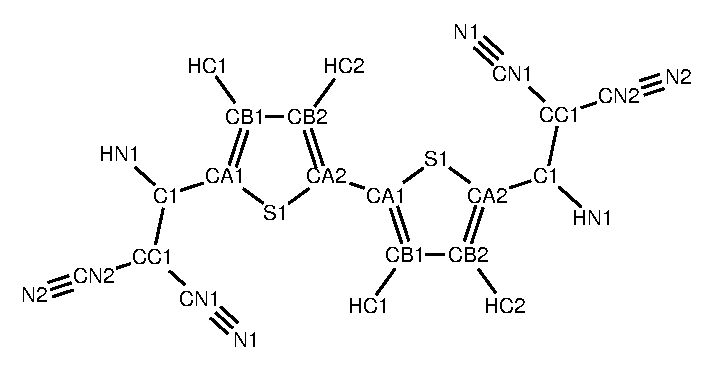
\includegraphics[width=0.45\textwidth]{./fig/chemical_structure/dcv2t_atom_types}\,
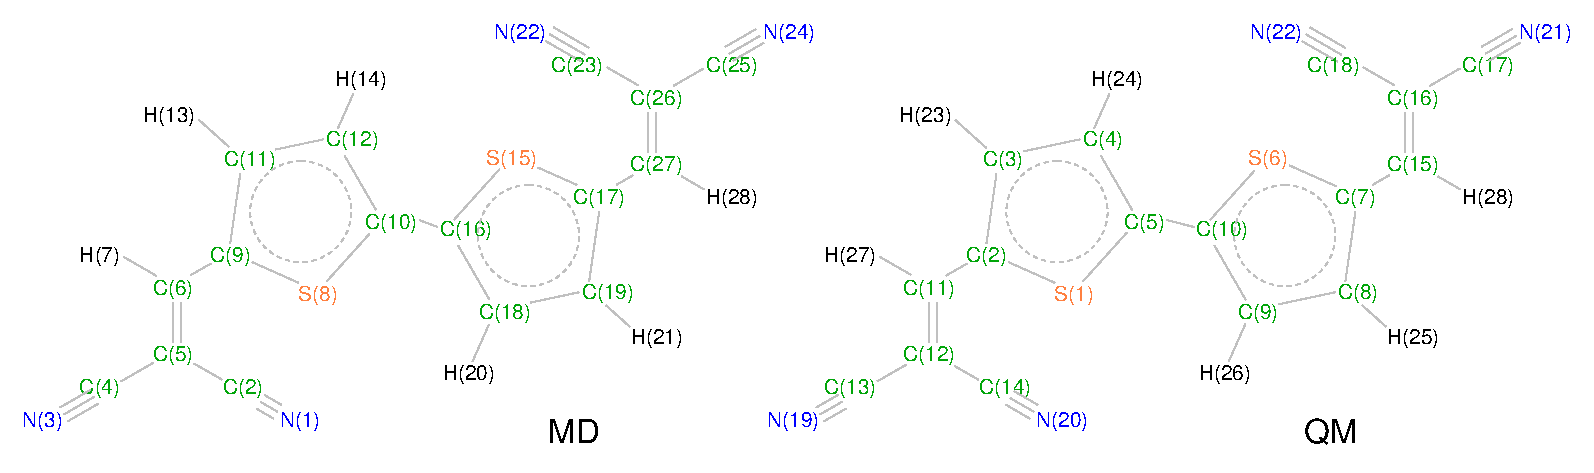
\includegraphics[width=0.45\textwidth]{./fig/chemical_structure/dcv2t_gaussian}
\caption{\small (a) \dcvt with atoms labelled according to \texttt{residue\_number:residue\_name:atom\_name}. There are four residues and two residue types: thiophene (THI) and dicyanovinyl (NIT). The corresponding pdb file is shown in listing~\ref{list:pdb}. (b) Atom numbering is used to split conjugated segments on rigid fragments and to link atomistic and quantum descriptions.}
\label{fig:dcv2t}
\end{figure}

\lstinputlisting[
  language=XML,
  basicstyle=\ttfamily\footnotesize,
  stringstyle=\ttfamily\footnotesize,
  showstringspaces=false,
  frame=lines,
  label=list:pdb, 
  morekeywords={HETATM,THI,NIT},
  caption={\small pdb file of \dcvt.}]%
{./fig/chemical_structure/dcv2t.pdb}

\section{Mapping file}
\label{sec:xmlmap}

The mapping file (referred here as \xmlcsg) is used by the program \ctpmap to convert an atomistic trajectory to a coarse-grained one. The coarse-grained trajectory contains positions, names, types, and orientations of rigid fragments. \xmlcsg contains definitions of rigid fragments (coarse-grained beads) and identifies to what conjugated segment a particular rigid fragment belongs. The description of the mapping options is given in table \ref{tab:map}. An example of \xmlcsg for a \dcvt molecule is shown in listing~\ref{list:map}. 

\begin{table}[ht]
\label{tab:map}
\caption{Description of the \xml mapping file (\xmlcsg).}
\rowcolors{1}{invisiblegray}{white} {\footnotesize \input{reference/xml/map.xml}}
\end{table}
\vfill
% Define new language for listings.
\lstdefinelanguage{MXML} {
   basicstyle=\ttfamily\scriptsize,
   sensitive=true,
   morecomment=[s][\color{gray}\rmfamily\itshape]{<!--}{-->}, 
   showstringspaces=false,
   numberstyle=\scriptsize,
   numberblanklines=true,
   showspaces=false,
   breaklines=true,
   showtabs=false,
   alsoletter={:},
   keywords = [1]
   { name,cg_molecule,cg_beads,cg_bead,crgunitname,bead,beads,type,topology,name,ident,maps,map,mapping,weights,position,qm,symmetry },
   keywordstyle={[1]\color{blue}},
}
\lstinputlisting[
 language=MXML,
 label=list:map,
 caption={Examle of \xmlcsg for \dcvt. Each rigid fragment (coarse-grained bead) is defined by a list of atoms. Atom numbers, names, and residue names should correspond to those used in \gromacs topology (see the corresponing listing \ref{list:pdb} of the pdb file).}]%
{./input/dcv2t/map.xml}

\clearpage
\section{Conjugated segments and rigid fragments}

Conjugated segments are described in a separate \xml file. An example for \dcvt is shown in listing~\ref{list:conjugated_segments}.



\clearpage
\begin{figure}[ht]
\centering
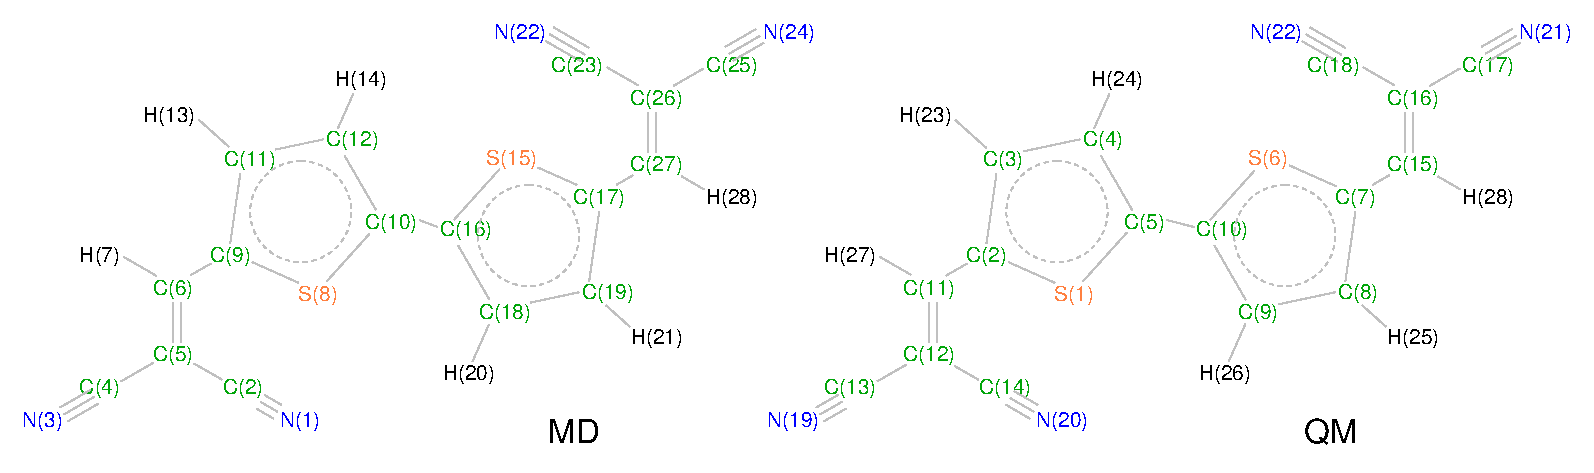
\includegraphics[width=\textwidth]{./fig/chemical_structure/dcv2t_gaussian} 
\caption{\small Atom order of \dcvt in the atomistic topology (MD) and qunatum chemical calculations (QM). The  link between two is established in the description of a conjugated segment shown in listing~\ref{list:conjugated_segments}.}
\label{fig:dcv2t_qm}
\end{figure}

\lstset{
  language=XML,
  frame=lines,
  basicstyle=\ttfamily\footnotesize,
  identifierstyle=\color{red},
  keywordstyle=\color{blue},
  showstringspaces=false,
  columns=fullflexible,
  commentstyle=\color{gray}\rmfamily\itshape,
  morekeywords={crgunit_type,ChargeUnitType,posname,orbname,basisset,transorb,reorg,nameneutr,namecrg,energy,beadconj,molname,name,monomer_atom_map,monomer_atom_weights},
}

\lstinputlisting[
 label=list:conjugated_segments, 
 caption={\small \xml file describing conjugated segments.
}]%
{./input/segments.xml}
\clearpage


\section{Molecular orbitals}
If the semi-empirical method is used to calculate electronic coupling elements, molecular orbitals of all molecules must be supplied. They can be generated using \gaussian program. The \gaussian input file for \dcvt is shown in listing~\ref{list:zindo_orbitals}. Provided with this input, \gaussian will generate \texttt{fort.7} file which contains the molecular orbitals of a \dcvt. This file can be renamed to \texttt{\dcvt.orb}. Note that the order of the atoms in the input file and the order of coefficients should always match. Therefore, the coordinate part of the input file must be supplied together with the orbitals. We will assume the coordinates, in the format \texttt{atom\_type: x y z}, is saved to the \texttt{\dcvt.xyz} file.

\attention{Izindo requires the specification of orbitals for hole and electron transport in \xmlcsg. They are the HOMO and LUMO respectively and can be retrieved from the \texttt{log} file from which the \texttt{\dcvt.orb} file is generated. The number of \texttt{alpha electrons} is the HOMO, the LUMO is HOMO+1 } 

\lstinputlisting[
 label=list:zindo_orbitals, 
 basicstyle=\ttfamily\footnotesize,
 morekeywords={chk,mem,punch,int,S,C,S,N,H},
 showstringspaces=false,
 keepspaces=true,
 caption={\small \gaussian input file \texttt{get\_orbitals.com} used for generating molecular orbitals. The first line contains  the name of the check file, the second the requested RAM. 
%
 \texttt{int=zindos} requests the method ZINDO, \texttt{punch=mo} states that the molecular orbitals ought to be written to  the \texttt{fort.7} file, \texttt{nosymm} forbids use of symmetry and is necessary to ensure correct position of orbitals with respect to the provided coordinates. The two integer numbers correspond to the charge and multiplicity of the system: $0\, 1$ corresponds to a neutral system with a multiplicity of one. They are followed by the types and coordinates of all atoms in the molecule.
}]%
{./input/get_orbitals.com}
%


\section{DFT transfer integrals}
\lstinputlisting[
  language=XML,
  label=list:TI_xml,
  stringstyle=\ttfamily\footnotesize,
  showstringspaces=false,
  caption={\small Example {\tt TI.xml} file created as the output of a \dipro calculation. Due to slightly different implementations, the orbitals indices refer to monomer indices in a \gaussian run but to indices in the merged dimer guess in a \turbomole run.}] {./input/TI.xml}




\chapter{Manual pages}

\section{Programs}
\label{ref:programs}
\input{reference/programs/all}

\section{Calculators}
\label{ref:caclulators}
\input{reference/calculators/all}

\section{Options}
\label{ref:options}
\input{reference/xml/ctp_listcharges.xml}



\appendix
\newcommand{\indM}{l} 
\newcommand{\indN}{m}
\newcommand{\lb}[1]{\langle #1 |}
\newcommand{\rb}[1]{| #1 \rangle}
\newcommand{\rbt}[1]{ #1 \rangle}

%\appendixpage
%\addappheadtotoc
\chapter{Bimolecular electron transfer rate}

\begin{figure*}[ht]
%    \includegraphics[width=1.0\textwidth]{fig/jortner_rate/marcus_parabolas_new}
   \caption{
(a) Potential energy surfaces of the charge transfer complex in a dimer representation. ET is from molecule $i$ to molecule $j$. In the initial state, $\rb{I_{00}}$, both molecules are in their vibrational ground states. In the final state, $\rb{F_{l'm'}}$, the neutral molecule $i$ is in vibrational state $l'$, while the charged molecule $j$ is in vibrational state $m'$. Initial and final states are coupled to a classical harmonic outer-sphere normal mode with mass weighted average coordinate $q$ and reorganization energy $\lambda_{ij}^\text{out}$. For small couplings $V_{I_{00}F_{l'm'}}$ the ET reaction takes place on the diabatic states (solid curves). 
%
(b) PES of molecule $i$ as a function of the averaged normal mode $q_i$. $l$ and $l'$ enumerate vibrational modes of the initial charged and the final neutral states. (c) Same as (b) for initially neutral molecule $j$. 
%
$\Delta U_i$ ($\Delta U_j$) is the internal energy difference while $\lambda_i^{cn}$ ($\lambda_j^{nc}$) is the  intramolecular reorganization energy for discharging molecule $i$ (charging molecule $j$). }
   \label{fig:marcus_parabolas}
\end{figure*}

In the case of a bimolecular electron transfer (ET) reaction the electron moves between two independent molecules. Therefore, one needs separate sets of coordinates for the donor and acceptor. Strictly speaking, the classical Marcus rate assumes a common set of vibrational coordinates and, as such, can not be used for bimolecular ET. Yet if the independent vibrational modes are harmonic, are treated classically, and the charging and discharging reorganization energies of the molecule are identical, one still obtains the Marcus-type ET rate with the intramolecular reorganization energy which is the sum of the reorganization energies of the donor and the acceptor~\cite{may_charge_2003}. Similarly, the classical treatment of the outer-sphere mode, which is due to rearrangement of the surrounding, allows to add its reorganization energy  to the intramolecular one.

However, the main issue with the classical Marcus rate is that the high-frequency intramolecular vibrational modes are energetically comparable to the C-C bond stretching mode. At room temperature $\hbar \omega_\text{CC} \sim 0.2\, \unit{eV} \gg k_\text{B}T \sim 0.025\, \unit{eV}$  and therefore these modes should be treated quantum mechanically. In fact, for a common set of intramolecular high-frequency  (quantum-mechanical) and an outer sphere low-frequency (classical) vibrational coordinates, a mixed quantum-classical multi-channel generalization of the Marcus formula is readily available~\cite{may_charge_2003}. Such generalization,  to the best of our knowledge, has not been made for the bimolecular ET rate, which requires independent sets of coordinates for donor and acceptor. The purpose of this section is to derive a quantum-classical expression for the ET rate with two independent, high-frequency vibrational modes and a common low-frequency outer sphere mode. 

Following Ref.~\cite{bredas_charge-transfer_2004} we assume that all intramolecular modes of a donor $i$ can be averaged into a mode with mass weighted coordinate ${q_i}$ and energy $\hbar\omega^{n}_i$ ($\hbar\omega^{c}_i$) for the molecule in a neutral (charged) state. Similar assumptions are made for the acceptor $j$. In addition, we allow for an averaged classical outer-sphere mode with mass weighted coordinate ${q}$ and energy $\hbar\omega^\text{out}_{ij}\ll k_\text{B}T$. This mode is common to both molecules and plays the role of the ET reaction coordinate~\cite{note_outer}.

In amorphous organic semiconductors the electronic coupling is usually small compared to both the energy of the classical vibrational mode and intermolecular reorganization energies. In this case the initial, $ \rb{I_{\indM\indN}}$, and final, $\rb{F_{\indM'\indN'}}$, states of the ET reaction are diabatic (non-interacting) dimer states which depend on the vibrational states (with quantum numbers $\indM, \indN, \indM, '\indN'$) of both molecules. The potential energy surfaces (PES) corresponding to these states are shown in \fig{marcus_parabolas}a. The PES for intramolecular degrees of freedom for molecules $i$ and $j$ are shown in \fig{marcus_parabolas}b and c, respectively.

For the contributions of the outer-sphere mode to initial and final states we introduce Hamiltonian functions
\begin{equation}
 H_{I,F}(q)=\frac{1}{2}\left[ \omega^\text{out} \left( q-q_{I,F} \right) \right]^2 \, ,
\end{equation}
where the equilibrium position in the initial (final) state $q_I$ ($q_F$) corresponds to the arrangement of all nuclear coordinates of molecules surrounding the ET complex when molecule $i$ ($j$) is charged.  The outer sphere reorganization energy, defined as $\lambda^\text{out}_{ij}=\frac{1}{2}\left[ \omega^\text{out}|q_I-q_F| \right]^2$,  is shown in~\fig{marcus_parabolas}a. It can be computed from the initial and final electric displacement fields of the charge-transfer complex. 

The complete Hamiltonian of the ET complex can now be written as
\begin{equation}
\begin{split}
 H_{ij}=&\hphantom{+}\sum_{\indM,\indN=0}^\infty \left( H_I(q) + E^{ij}_{\indM\indN} \right) \rb{I_{\indM\indN}} \lb{I_{\indM\indN}} %\\
        +\sum_{\indM',\indN'=0}^\infty \left( H_F(q) + E^{ji}_{\indN'\indM'} \right) \rb{F_{\indM'\indN'}} \lb{F_{\indM'\indN'}} %\\
        +\sum_{\indM,\indN,\indM',\indN'}V_{I_{\indM\indN}F_{\indM'\indN'}} \rb{I_{\indM\indN}} \lb{F_{\indM'\indN'}} +\text{h.c} \,, \\
 E^{ij}_{\indM\indN}=& \hphantom{+} U_i^{cC} + U_j^{nN} + E_i^\text{el} + E_i^\text{ext}
+ \hbar\left[\omega_i^c\left(\indM+\frac{1}{2}\right) + \omega_j^n\left(\indN+\frac{1}{2}\right) \right] \, , 
       \\
 E^{ji}_{\indN'\indM'}=&\hphantom{+} U_j^{cC} + U_i^{nN} + E_j^\text{el} + E_j^\text{ext} 
+ \hbar\left[\omega_j^c\left(\indN'+\frac{1}{2}\right) +\omega_i^n\left(\indM'+\frac{1}{2}\right)\right] \, .
\end{split}
\label{equ:hami}
\end{equation}
Here, a manifold of initial states, $\rb{I_{\indM \indN}} $, with quantum numbers $\indM$ ($\indN$) for intramolecular vibrations in molecule $i$ ($j$) and energy $E^{ij}_{\indM \indN}$, is coupled to a classical phonon bath $H_I(q)$. Transitions to the manifold of final states  $\rb{F_{\indM' \indN'}} $ where the charge has hopped from $i$ to $j$ are possible due to a coupling $V_{I_{\indM\indN}F_{\indM'\indN'}} $.
The initial, $E^{ij}_{\indM\indN}$,  and final, $E^{ji}_{\indN'\indM'}$, energies contain internal energies $U_i^{nN}$ and $U_i^{cC}$ ($U_j^{nN}$ and $U_j^{cC}$) of molecule $i$ (molecule $j$) in the neutral and charged ground states, the contributions of the external electric field, $E_i^\text{ext}$ and $E_j^\text{ext}$, and electrostatic interactions, $E_i^\text{el}$ and $E_j^\text{el}$, and respective oscillator energies.  

Within the Born-Oppenheimer approximation, a separation in terms of electronic and nuclear degrees of freedom gives
\begin{equation}
\begin{split}
 \rb{I_{\indM\indN}}&=\rb{\phi_i^c}\rb{\chi_{i\indM}^c}\rb{\phi_j^n}\rb{\chi^n_{j\indN}}\, ,\\
 \rb{F_{\indM'\indN'}}&=\rb{\phi^n_i}\rb{\chi^n_{i\indM'}}\rb{\phi_j^c}\rb{\chi_{j\indN'}^c}\, ,
\end{split}
\end{equation}
where $\phi_i^n$ ($\phi_i^c$) corresponds to the electronic part of the wave function, while $\chi_{i\indM}^n$  ($\chi_{i\indM}^c$) represents an $\indM$-th phonon mode of the neutral (charged) molecule $i$.

The coupling element $V_{I_{\indM\indN}F_{\indM'\indN'}}$ in~\equ{hami} can then be factorized in an electronic and nuclear parts 
\begin{equation}
V_{I_{\indM\indN}F_{\indM'\indN'}}=J_{ij} \lb{\chi_{i\indM}^c}\rbt{\chi_{i\indM'}^n} \lb{\chi_{j\indN}^n}\rbt{\chi_{j\indN'}^c}\,.
\end{equation}
Franck-Condon overlap integrals $\lb{\chi_{i\indM}^c}\rbt{\chi_{i\indM'}^n}$ ($\lb{\chi_{j\indN}^n}\rbt{\chi_{j\indN'}^c} $) describe couplings of vibrational modes $\indM,\indM'$ ($\indN,\indN'$) of the charged and neutral configurations of molecule $i$  ($j$). Exemplary modes are shown in~\fig{marcus_parabolas}b,c.

Since $k_\text{B}T\ll \hbar\omega_i^{c},\hbar\omega_j^{n}$ one can restrict the initial state to the vibrational ground-states $\indM=\indN=0$ while allowing tunneling to all vibrationally excited states $\indM'$ for molecule $i$ and $\indN'$ for molecule $j$. In other words, a single initial state $\rb{I_{00}}$ couples to a manifold of final states $\rb{F_{\indM',\indN'}}$. 
%
This assumes that ET is sufficiently slow compared to the relaxation of the intramolecular degrees of freedom, so that there is enough time for a complex to relax to its vibrational ground state between two consecutive ETs. 

The energy difference driving the reaction to channel ${\indM'\indN'}$  therefore is
\begin{equation*}
 \Delta E^{ij}_{\indM'\indN'}= E^{ij}_{00}-E^{ji}_{\indN'\indM'}=\Delta E_{ij} - \hbar (\omega_i^n\indM'+\omega_j^c\indN')\,,
\end{equation*}
where $\Delta E_{ij}=\Delta E_{ij}^\text{ext}+\Delta E_{ij}^\text{el}+\Delta E^\text{int}_{ij}$.

Assuming that $|V_{I_{00}F_{\indM'\indN'}}|\ll\lambda_{ij}^\text{out},\hbar\omega^\text{out}$ and using Fermi's golden rule with $V_{I_{00}F_{\indM'\indN'}}$ as a perturbation to the initial diabatic state, we obtain a multi-channel rate equation
\begin{equation}
%\begin{split}
\omega_{ij}=\sum_{\indM',\indN'=0}^\infty \frac{2\pi}{\hbar}|V_{I_{00}F_{\indM'\indN'}}|^2 
% \times  
\int dq f_I(q) \delta(\Delta E^{ij}_{\indM'\indN'} + H_I(q) -H_F(q))\, .
%\end{split}
\end{equation}
where the thermal averaging over the classical outer-sphere mode is performed by introducing a  canonical distribution function  $f_I(q)=Z^{-1}\exp(-H_I(q)/k_\text{B}T)$, with $Z=\int{dq \exp(-H_I(q)/k_\text{B}T)}$.

Energy conservation pins the transition to the crossing point of the diabatic PES (see~\fig{marcus_parabolas}a) resulting in 
\begin{eqnarray}
 \omega_{ij}= \frac{2\pi}{\hbar}  \frac{|J_{ij}|^2}{\sqrt{4\pi \lambda_{ij}^\text{out} k_\text{B}T}} 
 \sum_{\indM',\indN'=0}^\infty
 |\lb{\chi_{i0}^c}\rbt{\chi_{i\indM'}^n}|^2 |\lb{\chi_{j0}^n}\rbt{\chi_{j\indN'}^c}|^2 
%\nonumber \\&& 
\exp
\left\{ -\frac{ \left[ \Delta E_{ij}-\hbar(\indM'\omega_i^n+\indN'\omega_j^c) -\lambda_{ij}^\text{out} \right]^2}{4\lambda_{ij}^\text{out} k_\text{B}T}
\right\} .
\label{equ:jjortner}
\end{eqnarray}
\Equ{jjortner} is the quantum-classical expression for the bimolecular ET rate with two independent, high-frequency vibrational modes and one classical common outer-sphere mode. It is the main result of this section. 

If the curvatures of intramolecular PES of charged and neutral states of a molecule are different, that is $\omega_i^c\neq\omega_i^n$, the corresponding reorganization energies, $\lambda_i^{cn}=\frac{1}{2}[\omega_i^n(q_i^n-q_i^c)]^2$ and $\lambda_i^{nc}=\frac{1}{2}[\omega_i^c(q_i^n-q_i^c)]^2$, will also differ. In this case the Franck-Condon (FC) factors for discharging of molecule $i$ read \cite{chang_new_2005}
\begin{equation}
%\begin{split}
%&
|\lb{\chi_{i0}^c}\rbt{\chi_{i\indM'}^n}|^2 = 
\frac{2}{2^{l'}l'!} \frac{\sqrt{\omega_i^c\omega_i^n}}{(\omega_i^c+\omega_i^n)} \exp\left( -|s_i| \right)
%\nonumber \\
%& \times
 \left[ \sum_{\substack{k=0\\k\,\text{even}}}^{\indM'} {\indM' \choose k} 
\left( \frac{2 \omega_i^c }{\omega_i^c+\omega_i^n}\right)^{k/2} \frac{k!}{(k/2)!}
H_{\indM'-k} \left( \frac{s_{i}}{\sqrt{2S^{cn}_i}}\right) 
\right]^2
\, ,
%\end{split}
\end{equation}
where $H_n(x)$ is a Hermite polynomial, $s_i=\frac{2\sqrt{\lambda_i^{nc}\lambda_i^{cn}}}{\hbar(\omega_i^c+\omega_i^n)}$, and $S^{cn}_i=\lambda_i^{cn}/\hbar\omega_i^c$. The FC factors for charging of molecule $j$ can be obtained by substituting $(s_i,S^{cn}_i,\omega_i^c)$ with $(-s_j,S^{nc}_j, \omega_j^n)$. In order to evaluate the FC factors, the internal reorganization energy $\lambda_i^{cn}$ can be computed from the intramolecular PES, as shown in~\fig{marcus_parabolas}b,c. 

To conclude the section, we compare the bimolecular quantum-classical rate, \equ{jjortner}, the classical bimolecular Marcus rate, eq.~(1) of the main text, and the quantum-classical Jortner rate with a common set of vibrational coordinates~\cite{may_charge_2003}
\begin{eqnarray}
 \omega_{ij} = \frac{2\pi}{\hbar}  \frac{|J_{ij}|^2}{\sqrt{4\pi \lambda_{ij}^\text{out} k_\text{B}T}} 
 \sum_{N=0}^\infty \frac{1}{N!} \left( \frac{\lambda_{ij}^\text{int}}{\hbar\omega^\text{int}} \right)^{N} 
  \exp \left( - \frac{\lambda_{ij}^\text{int}}{\hbar\omega^\text{int}}\right) 
%\nonumber\\&& 
\exp
\left\{ -\frac{ \left[ \Delta E_{ij}-\hbar N\omega^\text{int} -\lambda_{ij}^\text{out} \right]^2}{4\lambda_{ij}^\text{out} k_\text{B}T}
\right\} .
\label{equ:jortner}
\end{eqnarray}

If $\omega_i^c=\omega_i^n=\omega_i$ ($\lambda_i^{nc}=\lambda_i^{cn}=\lambda_i$), the Franck-Condon factor simplifies to
\begin{equation}
|\lb{\chi_{i0}}\rbt{\chi_{i\indM'}}|^2 = \frac{1}{\indM'!} \left( \frac{\lambda_i}{\hbar\omega_i} \right)^{\indM'} \exp \left( - \frac{\lambda_i}{\hbar\omega_i}\right)\,.
\end{equation}
If this simplification is applicable for both donor and acceptor molecules,  \equ{jjortner} becomes identical to the quantum-classical rate~\equ{jortner} with $\lambda_{ij}^\text{int}=\lambda_i+\lambda_j$.

\begin{figure*}[ht]
%   \includegraphics[width=\linewidth]{fig/jortner_rate/compare_rates}
   \caption{ (a) Scaled hopping rates, $\bar{\omega}_{ij} = \omega_{ij}  J_{ij}^{-2} (2\pi)^{-1} \hbar\sqrt{4\pi k_\text{B}T}$, calculated using the classical Marcus, Jortner quantum mechanical~\equ{jortner} and bimolecular multichannel~\equ{jjortner} rate expressions. 
%
Outer sphere reorganization energy $\lambda_{ij}^\text{out}=0.05\, \unit{eV}$,  $\lambda^{cn}_i=\lambda_j^{cn}=0.14\, \unit{eV}$, and $\lambda^{nc}_i=\lambda^{nc}_j=0.09\, \unit{eV}$ (all added in the classical Marcus rate while the latter two are added for the Jortner rate). 
%
Intramolecular vibrations have averaged frequency $\hbar\omega_i^\text{int}=\hbar\omega_j^\text{int}=0.2\, \unit{eV}$ for the Jortner rate while $\hbar\omega_i^n=0.2\, \unit{eV}$ and $\hbar\omega_j^c=\hbar\omega_i^n \sqrt{\lambda_j^{nc}}/\sqrt{\lambda_j^{cn}}$ for the bimolecular rate. 
%
(b) The same but for $\lambda_{ij}^\text{out}=0.1\, \unit{eV}$. 
%
(c) Histogram of rates at a field of $10^8\, \unit{Vm^{-1}}$ for the Marcus and Jortner rates with distance dependent $\lambda_{ij}^\text{out}<0.08\, \unit{eV}$ for the neighborlist pairs and constant $\lambda^\text{int}=0.23\, \unit{eV}$. A small difference can be seen in the tail of small rates.}
   \label{fig:mj_comparison}
\end{figure*}

% discussion of the equation
To compare the quantum-mechanical and classical rates, intramolecular hole reorganization energies of \Alq, $\lambda^{cn}_i=0.14\,\unit{eV}$ and $\lambda^{nc}_i=0.09\,\unit{eV}$ were used. We also assumed that $\omega_i^n=0.2\,\unit{eV}$ and $\omega_i^c=\omega_i^n\sqrt{\lambda^{nc}_i / \lambda^{cn}_i}$. Due to the uncertainty in determining $\lambda_{ij}^\text{out}$, two cases are considered, $\lambda_{ij}^\text{out}=0.05\,\unit{eV}$ (\fig{mj_comparison}a) and $\lambda_{ij}^\text{out}=0.10\,\unit{eV}$ (\fig{mj_comparison}b). Note that the estimate made in the main text predicts $\lambda_{ij}^\text{out} < 0.08\,\text{eV}$. In both cases we used fixed, molecular-separation independent, $\lambda_{ij}^\text{out}$. 

\Fig{mj_comparison} shows that the main difference between the quantum-classical and classical rates is the tail of smaller rates for large negative $\Delta E$ (endothermal hopping) and higher rates for large positive $\Delta E$ (exothermal hopping).  \Fig{mj_comparison}c also shows the corresponding distributions of rates for all pairs from the neighbor list for 512 molecules of  amorphous \Alq. Here we used the distance-dependent $\lambda_{ij}^\text{out}$ from the neighbor list as computed from dielectric displacement fields with the Pekar factor of $c_p=0.01$. One can see that the distributions are practically on top of each other (except for very small rates) and hence will lead to similar charge dynamics. 

In general, our observation is that for a situation with (i) intramolecular reorganization energy similar to the outer sphere one ($\lambda_{ij}^\text{int} \sim \lambda_{ij}^\text{out}$), (ii) driving force $\Delta E_{ij}$ small compared to the intramolecular reorganization energy, and (iii) $\lambda \sim \hbar \omega$, the classical (eq.~(1) of the main text) and semi-classical  (\equ{jortner} and \equ{jjortner}) expressions lead to quantitatively similar rates.
However, for systems with large $\Delta E_{ij}$, such as donor-acceptor mixtures, \equ{jjortner} or \equ{jortner} should be used. In this case a rather accurate estimate of the outer sphere reorganization energy is required~\cite{mcmahon_evaluation_2010}.


\chapter{Calculators}
\label{sec:calculators}

Calculator is a piece of code which computes specific system properties, such as site energies, transfer integrals, etc. \ctprun is a wrapper program which executes all calculators. The generic syntax is 
\begin{verbatim}
  ctp_run --exec "calc1, calc2, ..." --opt options.xml
\end{verbatim}
%
File \texttt{options.xml} lists all options needed to run a specific calculator. The format of this file is explained in listing~\ref{list:calc}. A complete list of calculators is given in the \refcalc reference section.
%
\lstinputlisting[label=list:calc, 
 caption={\small A part of the \texttt{options.xml} file with options for the \texttt{calculator\_name\{1,2\}} \refcalc.
}]{./appendix/calculators.xml}




\bibliographystyle{achemso}
\bibliography{literature_short}


\end{document} 
